\documentclass{article}
\usepackage{graphicx}
\usepackage[spanish]{babel}
\usepackage[utf8]{inputenc} % Ensures proper handling of special characters
\usepackage{amsthm}
\usepackage{amsmath}
\usepackage{amsfonts}
\usepackage{hyperref}
\usepackage{mathrsfs}
\usepackage[font=footnotesize,labelfont=bf,labelsep=colon]{caption} % Personalización de captions
\DeclareMathOperator*{\argmin}{arg\,min}
% Define the unnumbered theorem
\newtheorem{thm}{Teorema}[subsection]
\newtheorem{lem}{Lema}[subsection]
\newtheorem{cor}{Corolario}[thm]
\newtheorem{dfn}{Definición}[subsection]
\newtheorem{obs}{Observación}[subsection]

%\newtheorem*{def}{Definicion}

\begin{document}


\title{Teoría del Aprendizaje Estadístico}
\author{Nicolas Silva Nash \\ Departamento de Matemática \\ Universidad Nacional del Comahue}
%\date{\today}
\maketitle

\section{Introducción}
La Teoría del Aprendizaje Estadístico proporciona la base teórica para muchos de los algoritmos de aprendizaje automático actuales y,
sin lugar a dudas, es una de las ramas más bellamente desarrolladas de la inteligencia artificial en general. Nació con el perceptrón de Rossenblat
y la escuela matemática de la Unión Soviética en la década de 1960, y ganó amplia popularidad en la década de 1990 tras el desarrollo de las llamadas 
Máquinas de Vectores de Soporte (\textit{SVM}, por sus siglas en inglés), que se han convertido en una herramienta estándar para el reconocimiento de 
patrones en muchas disciplinas, que van desde la visión por computadora hasta la biología computacional.\\

Proporcionar la base para nuevos algoritmos de aprendizaje no ha sido la única motivación para desarrollar la Teoría del Aprendizaje 
Estadístico. También ha sido una gesta de caracter filosófico, en el intento de responder a la pregunta de qué nos permite extraer conclusiones válidas 
a partir de datos empíricos.  

\section{El aprendizaje}

En este contexto, el \textit{aprendizaje} es el proceso a través del cual pueden inferirse reglas generales a partir de ejemplos. Nos interesa 
entender como una máquina -una computadora- puede resolver ciertos problemas sin conocer las reglas de antemano, solo a partir de ejemplos y a través
de un \textit{algoritmo de aprendizaje}. El objetivo es que la máquina pueda no solo aprender a reconocer las reglas que rigen a los ejemplos dados,
si no que también pueden generalizar dichas reglas para ejemplos que le serán presentados con posterioridad.\\

Llamamos a esta disciplina \textit{aprendizaje automático} (en inglés, \textit{Machine Learning}, literalmente ``aprendizaje de máquinas") y reconocemos
sus raíces en otras disciplinas: Estadística Matemática, Ciencias de la Computación e Inteligencia Artificial. Si bien el aprendizaje suele ser una
parte fundamental de la mayoría de los esfuerzos en materia de Inteligencia Artificial, el objetivo del Machine Learning es más acotado que el de su 
rama madre: En vez de intentar definir, explicar o generar comportamiento inteligente o \textit{inteligencia}, aquí nos interesa solamente descubrir los mecanismos
a través de los cuales las computadoras pueden resolver algunas tareas acotadas y bien definidas, y que en general escapan a soluciones que pueden
ser especificadas con una cantidad finita de código de programación (reglas determinísticas). \\

Con fines ilustrativos, nos centraremos primero en el más conocido de los problemas del Machine Learning, el de clasificación. Consideremos dos espacios
de variables: \(X\), llamado \textit{espacio de entrada}, e \(Y\), el  \textit{espacio de etiquetas}. En un problema de clasificación, deseamos poder etiquetar
correctamente elementos de \(X\) con los valores de \(Y\). Por ejemplo, podríamos querer clasificar un conjunto de datos, en alguna representación fija, de distintos 
objetos en una cantidad de etiquetas como: silla, cama, microondas, perro, gato. Si esta representación es en imágenes de \(N\times M\) pixeles en blanco y negro (realmente, 
matrices de orden \(N\times M\) con coeficientes reales en el interavalo \([0,1]\) que representan la intensidad de cada pixel, del negro al blanco), el espacio \(X\) es 
el conjunto de dichas matrices y el espacio \(Y\) las categorías distintas que corresponden a lo que las imágenes muestran. Con el fin de aprender, a un algoritmo se le 
muestran ejemplos de imágenes y sus respectivas etiquetas \((X_1,Y_1)\), \((X_2,Y_2)\), ..., \((X_n,Y_n)\), a partir de los cuales este debe encontrar una función
\(f: X\rightarrow Y\), que comete la menor cantidad de errores posibles. A esta función \(f\) la llamamos \textit{clasificador}.

\section{La historia del aprendizaje automático}

El primer modelo de aprendizaje automático, según Vapnik en [2], fue sugerido por F. Rosenblatt, un psicólogo estadounidense, al que llamó \textit{perceptrón}, y su introducción
constituye el comienzo del análisis matemático del aprendizaje. Conceptualmente, la idea del perceptrón no era nueva, estando presente en la litetura de Neurofisiología durante
varios años. Rosenblatt, sin embargo, se aventuró en describir el modelo como un programa para computadoras y demostró con simples experimentos que dicho modelo era generalizable.
El perceptrón fue construído como una solución a un problema particular dentro del aprendizaje automático, el reconocimiento de patrones. En el caso más sencillo, este problema
consiste en hallar una regla para separar datos en dos categorías distintas a partir de ejemplos.\\

Para construir la regla de separación, el perceptrón sigue el modelo más sencillo de neurona, propuesto previamente por McCulloch y Pitts, de acuerdo al cual una neurona recibe
\(n\) valores (o \textit{inputs}) en la forma de un vector \(x = (x^1,\dots, x^n) \in X \subset \mathbb{R}^n \) y genera una etiqueta (\textit{output}) 
\(y\in\{-1,+1\}\) a través de una dependecia funcional dada por
\[
y = sgn\{(w\cdot x)-b\}
\]

con \(\cdot\) el producto interno de vectores en \(\mathbb{R}^n\), \(b\) un valor de límite y un vector \(w\) que se genera en el proceso de aprendizaje. Geométricamente, una 
neurona divide el espacio \(X\) en dos regiones: en una la etiqueta \(y\) vale \(+1\) y en la otra \(-1\). Las dos regiones son separadas por el hiperplano:
\[
(w\cdot x) - b = 0
\]


El vector \(w\) y el escalar \(b\) determinan la posición del hiperplano y sus valores son aprendidos por el perceptrón. Cuando combinamos varias neuronas, el perceptrón
separa el espacio de entrada en en dos regiones lineales a trozos y no necesariamente conexas. En 1960 no era claro como elegir todos los parametros \((w_1,\dots,w_k)\) y
\((b_1,\cdots, b_k)\) de todas las neuronas, por lo que se fijaban los valores de las primeras \(k-1\) y se intentaba encontrar los valores deseables para la última
de ellas. Geométricamente, se transformaba el espacio de entrada $X$ en un nuevo espacio $Z$ (eligiendo coeficientes apropiados para las primeras $k-1$ neuronas) y luego
se utilizaban los datos de entrenamiento para construir un hiperplano que separe el plano $Z$.
Tomando prestados de la fisiología los conceptos de aprendizaje con estímulos de premios y castigos, Rosenblat propuso un simple algoritmo para hallar estos 
coeficientes de manera iterativa, el cual describiremos a continuación.

DESCRIBIR perceptrón.\\

En 1962 Novikoff demostró el primer teorema relacionado al perceptrón. Podemos decir que este teorema inció propiamente la teoría del aprendizaje.

\begin{thm}
Dado un conjunto de datos de entrenamiento como el descrito previamente, de manera que\\
1) La norma de los vectores de entrenamiento $z_i$ está acotada por una constante $R$:
$$
|z_i| \leq R, \qquad \forall i=1,2,\dots,k
$$
2) Los datos de entrenamiento pueden separados con un margen $\rho$:
$$
\sup_{w} \min_{i} y_i(z_i\cdot w) > \rho
$$
3) Los datos son alimentandos al perceptrón una cantidad \textit{suficiente} de veces.\\

Entonces el algoritmo encuentra el hiperplano que separa los datos de entrenamiento, luego de a lo
sumo $N$ correcciones, con $N$ verificando:
$$
N \leq \left [ \frac{R^2}{\rho^2}\right ]
$$

\end{thm}

Resaltamos este teorema porque jugó un papel fundamental en la creación de la teoría del aprendizaje, conectando el
principio de minimización de errores en el conjunto de datos de entrenamiento con la capacidad de generalización
de los algoritmos de clasificación y su causa.

\section{Hacia la formalización}

Volviendo al caso de clasificación binaria en aprendizaje supervisado, partimos de ejemplos (datos de entrenamiento) 
en un espacio de entrada $X$ con alguna de las dos posibles etiquetas del espacio $Y=\{-1,+1\}$. Aquí, \textit{aprender}
se reduce a estimar una relación funcional $f:X\rightarrow Y$, el clasificador. Un algoritmo de aprendizaje es aquel
que a partir de los datos de entrenamiento construye una función $f$. Nos interesa construir una teoría que no asuma
de manera estricta nada acerca de $X$ e $Y$, pero nos permitimos asumir ciertas cosas del mecanismo que genera los
datos de entrenamiento. En particular, asumiremos que existe una \textit{distribución de probabilidad conjunta} $P=P(X,Y)$
sobre $X\times Y$ y que las muestras son tomadas de forma independiente de esta distribución de forma \textit{iid} -independiente
e idénticamente distribuída-. Notemos lo siguiente:
\begin{enumerate}
    \item \textit{No imponemos condiciones a la distribución de probabilidad $P$}. La gran diferencia que encontramos entre la Estadística
    tradicional y la teoría del aprendizaje estadístico es que en esta última trabajamos de manera agnóstica a la distribución
    que genera las muestras y deseamos llegar a conclusiones generales.
    \item \textit{Consideramos a las etiquetas de manera no determinística.} Consideramos a $P$ como una distribución de probabilidad
    no solo sobre las instancias de $X$, si no también sobre las propias etiquetas de $Y$. Por lo tanto, estas últimas no son solo 
    funciones tradicionales de los datos en $X$, si no que ellas mismas pueden ser aleatorias. Tenemos al menos dos buenas razones
    para tomar esta consideración: por un lado, el proceso de generación de datos puede tener ruido al asignar etiquetas (por ejemplo
    tomemos el caso de un detector de spam basado en la opinión de etiquetadores humanos que clasifican emails con un porcentaje de error; incluso
    los humanos pueden clasificar incorrectament algunos de esos emails), y por otro, ciertos problemas se prestan a que existan
    clases que se solapan (pensemos en la dificultad en diferenciar a un perro de un gato en una fotografías que los captura desde
    una gran distancia o con baja resolución).\\
    En la práctica, en vez de asignar etiquetas a los elementos en $X$ de manera determinística, daremos la probabilidad condicional
    de la etiqueta $y$ dado el valor $x$. En el caso de clasificación binaria, basta solo dar la probabilidad $P(Y=1|X=x)$ de que la etiqueta
    tenga valor $Y=1$, dado que la restante es complementaria:
    $$
    P(Y=-1|X=x) \quad = \quad 1 - P(Y=1|X=x)
    $$
    Ciertos problemas que hagan uso de datos con etiquetas con poco ruido nos llevaran naturalmente a probabilidades condicionales cercanas
    a $0$ y $1$, dejando un margen de error pequeño, pero cuando tratemos con solapamiento de clases, las probabilidades condicionales
    pueden acercarse a $\frac{1}{2}$ para cada etiqueta. Independientemente de la causa, que las probabilidades condicionales sobre
    las etiquetas se acerquen a $\frac{1}{2}$ vuelve más dificil el aprendizaje, dado que crece el número de errores del clasificador.
    \item \textit{Muestro independiente}. Una de las condiciones más fuertes que imponemos en la teoría del aprendizaje estadístico es
    que asumimos que las muestras son tomadas de forma independiente. En muchas aplicaciones, esta suposición está justificada, pero
    hay ramas muy importantes de la disciplina en donde esto no se cumple, por ejemplo en el análisis de series de tiempo, en donde
    la secuencialidad de los datos viola la condición de iid (cada valor depende en alguna medida de los anteriores). Esto es también 
    cierto para las aplicaciones a lenguaje natural, y constituye una de las razones principales por las cuales esta rama más moderna 
    del aprendizaje tiene bases teóricas menos fuertes que el aprendizaje automático tradicional.
    \item \textit{La distribución P es fija}. Al no considerar al tiempo como un parámetro, ni existir un orden en las muestras, asumimos
    que la distribución que las origina es siempre la misma. Esto, como en el punto anterior, no se cumple en las series de tiempo. Otro
    caso donde se viola esta suposición es en aquellos problemas en donde la distribución de probabilidad de los datos de entrenamiento no
    coincide con el de los datos posteriores, llamado \textit{covariate shift}, por ejemplo en un sistema de \textit{scoring} de usuarios
    de una empresa que crece súbitamente y que suma a personas que no se corresponden a los perfiles que existían originalmente en su base
    de datos (e.g. se admite que inmigrantes no bancarizados y sobre los que no hay datos previos accedan a préstamos).
    \item \textit{La distribución P es desconocida al momento de aprender}. Si conociéramos de antemano la probabilidad condicional $P$,
    el problema del aprendizaje sería trivial pues podríamos siempre determinar el mejor clasificador posible (aunque no sea perfecto,
    dada la naturaleza aleatoria de las etiquetas). Solo tenemos acceso a $P$ de manera indirecta, a través de las muestras. Intuitivamente,
    esto nos hace pensar que, consiguiendo un número lo suficientemente grande de muestras, podemos aproximar las propiedades de la distribución
    $P$, pero con errores. Uno de los principales logros de la teoría del aprendizaje estadístico es brindarnos un marco teórico para
    acotar este error.
\end{enumerate}

\subsection{Pérdida y Riesgo}

Para saber qué tan bien se comporta un clasificador $f$, necesitamos medir sus equivocaciones. Para esto, definiremos una \textit{función de pérdida},
$\ell$, que le asigne un valor al hecho de que $f$ clasifique a cierto $x\in X$ con la etiqueta $y\in Y$. Llamermos \textit{costo} a dicho valor, 
dado que más adelante penalizaremos al clasificador en base a los errores que cometa a través del alogritmo de aprendizaje.\\
El ejemplo más sencillo de función de pérdida es la ``pérdida-0-1'', que le asigna un costo de $0$ a una instancia de clasificación correcta y un costo
$1$ a una incorrecta, es decir:
$$
\ell(X,Y,f(X)):= \begin{cases}
    1 \qquad \text{si } f(X) \neq Y \\
    0 \qquad \text{si } f(X) = Y
\end{cases}
$$
En problemas de regresión, la función de pérdida más conocida es el \textit{error cuadrático}, dado por
$$
\ell(X,Y,f(X)):= (Y-f(X))^2
$$
Por convención, una pérdida igual a $0$ implica una clasificación perfecta y valores mayores implican peor clasificación. Es decir,
el aprendizaje suele implicar un desafío de optimización en dónde deseamos hallar el mínimo de la función de perdida.

Mientras que la función de pérdida mide el error del clasificador en un punto individual $x\in X$, llamamos \textit{riesgo}, $\mathcal{R}$, 
del clasificador a la pérdida esperada sobre todos los datos generados por la distribución de probabilidad $P$. Es decir
$$
\mathcal{R}(f) := \mathbb{E}\left( \ell(X,Y,f(X)) \right)
$$
Desde luego que otra función $g$ es un mejor clasificador que $f$ para un problema dado si su riesgo es más bajo, es decir si $\mathcal{R}(g)
< \mathcal{R}(f)$, por lo que el mejor clasificador de todos es aquel con el riesgo más bajo.\\

Algo que no hemos considerado aún es si los clasificadores $f$ tienen alguna característica especial. Para formalizarlo, tomaremos funciones de un
espacio de funciones $\mathcal{F}$ que aplican $X$ en $Y$. En un principio, parecería aceptable tomar el espacio de todas las funciones posibles, o 
más precisamente, el conjunto de todas las funciones \textit{medibles} que aplican $X$ en $Y$, $\mathcal{F}_{all} = \{f \text{ medibles  } | 
\; f: X \rightarrow Y \}$. En este caso, podemos señalar cuál es el clasificador ideal, dada la distribución $P$, al que llamamos
\textit{clasificador Bayesiano}, $f_{\text{Bayes}}$, y al que definimos como:
$$
f_{\text{Bayes}} := \begin{cases}
1 \qquad \; \; \text{  si } P(Y=1 | X=x) \geq \frac{1}{2}\\
-1 \qquad \text{en otro caso }
\end{cases}
$$

Observermos que, en caso de que las etiquetas fueran determinísticas, es decir donde $P(Y=y|X=x)=1$ para cada $x\in X$ con su
respectiva etiqueta $y$, $f_{\text{Bayes}}$ eligiría correctamente en todos los casos. De existir un ligero solapamiento de clases 
de tal manera que para un cierto $x$ tengamos $P(Y=1|X=x) = 0.9$, entonces tendríamos
que en la mayoría de los casos la etiqueta de $x$ es $+1$ y, siendo este el valor elegido por $f_{\text{Bayes}}$, el clasificador
Bayesiano estaría en lo correcto.\\

En la práctica no es posible computar directamente el clasificador Bayesiano dado que, como dijimos, la distribución de probabilidad
conjunta $P$ es desconocida. Sin embargo, este clasificador es una herramienta teórica que nos permite formular el problema
estandar de la clasificación binaria, el cual es:\\

\textit{Dado un conjunto de datos de entrenamiento $ \{ (X_1,Y_1),\dots,(X_n, Y_m)\}$ obtenidos iid de una distribución $P$, y dada una
función de pérdida $\ell$, deseamos construir una funión clasificadora $f:X\rightarrow Y$ cuyo riesgo $\mathcal{R}(f)$ sea lo
más cercano posible al riesgo de $f_{\text{Bayes}}$.}\\

Notemos que no solo es imposible computar el error del clasificador Bayesiano, sino también el propio riesgo de cualquier clasificador
$f$. Es decir, dado un problema definido (minimizar el riesgo del clasificador), con una solución ideal que podemos escribir (el propio
clasificador Bayesiano), no tenemos manera de computar ninguna cosa de utilidad. Aquí es donde la teoría de aprendizaje estadístico
nos permite llegar a resultados y obtener garantías de la utilidad de esas soluciones.

\subsection{Generalización}

Dado que no conocemos la distribución de probabilidad $P(X,Y)$, no podemos calcular la esperanza de la pérdida de un clasificador cualquiera
$f$, es decir su riesgo. Lo que si podemos hacer, dado un conjunto de entrenamiento, es ''contar" (o medir, en general, para problemas
que no son de clasificación binaria) el número de errores del clasificador sobre los datos de entrenamiento. A esta cantidad le daremos
el nombre de \textit{riesgo empírico} y lo veremos presente en la literatura también como \textit{error de entrenamiento}. Lo definimos
como
$$
R_{emp}(f) := \frac{1}{n} \sum_{i=1}^n \ell(X_i,Y_i,f(X_i))
$$

Por ejemplo, de la función de pérdida llamada error cuadrático se deriva el riesgo empírico \textit{error cuadrático medio}, que es ampliamente
utilizado en la práctica.

Usualmente, un algoritmo de aprendizaje aceptable es capaz de producir un clasificador $f$ que performa aceptablemente bien en un conjunto de datos
conocido, es decir tal que el riesgo empírico del clasificador es bajo. Nos interesa que un clasificador $f$ tenga riesgo bajo en todo el espacio
de entrada $X$, no solo en los datos de entrenamiento. Decimos que un clasificador \textit{generaliza} bien si la diferencia entre su riesgo
y su riesgo empírico es baja.\\

DEFINICIÓN Generalización\\

Por supuesto que una buena generalización no asegura que el riesgo, ni el riesgo empírico, sean bajos, si no que dichas cantidades son cercanas.
Pero lo que nos interesa es que el riesgo empírico sea un buen estimativo del riesgo del clasificador, y esto es lo que nos permitirá
hacer afirmaciones acerca del error del clasificador en la práctica.

\subsection{Consistencia}
Intuitivamente, parece razonable pedirle a un algoritmo de aprendizaje que, al ser presentado con más y más ejemplos, converja a una
solución óptima. En Estadística, la noción de \textit{consistencia} se relaciona con la capacidad de hacer afirmaciones con respecto a lo que
sucede en el límite de una cantidad infinita de muestras y, a diferencia de la generalización, que es acerca de una función en particular,
es una propiedad de un conjunto de funciones. Para ilustrar este concepto, denotemos como $f_n$ al clasificador construido por un algoritmo
de aprendizaje luego de ser presentado con $n$ puntos de entrenamiento. Por el momento no repararemos en cómo el algoritmo construye esta
función, pero podemos estar seguro que la elige de un cierto espacio funcional $\mathcal{F}$. Más adelante veremos que dicho espacio puede
estar explícitamente dado, como en el caso de la regresión lineal, o no, y existir implícitamente en el mecanismo del propio algoritmo,
como es el caso de las redes neuronales. Más allá de si $\mathcal{F}$ es explícito o no, el algoritmo debe elegir a la mejor función
en dicho espacio basándose en los puntos de entrenamiento. Por otro lado, sabemos precisamente cuál es en teoría el mejor clasificador 
en $\mathcal{F}$: el que tiene el menor riesgo. Por simplicidad, supongamos que este es único (no tiene por qué serlo, puede no haber
un solo mínimo global para la función de riesgo). Definimos a este clasificador óptimo como:
$$
f_{\mathcal{F}} = \argmin _{f\in{\mathcal{F}}} \mathcal{R}(f)
$$
Considerando que el clasificador bayesiano introducido en la sección anterior es el mejor clasificador posible, podríamos denotarlo,
siguiendo la misma convención, como $f_{\mathcal{F}_{all}}$. Desde luego que el espacio $\mathcal{F}$ que elegimos 
puede no contenerlo, por lo que $\mathcal{R}(f_{\text{Bayes}}) < \mathcal{R}(f_{\mathcal{F}})$. Con estas ideas, podemos definir
los distintos de convergencia que trataremos al considerar el concepto de consistencia.

\begin{dfn}
    Sea $(X_i,Y_i)_{i\in\mathbb{N}}$ una sucesión infinita de puntos de entrenamiento que han sido tomados iid de una distribución $P$.
    Sea $\ell$ una función de pérdida. Por cada $n\in \mathbb{N}$, sea $f_n$ un clasificador construído por algún algoritmo de aprendizaje
    usando los primeros $n$ puntos de entrenamiento. Sea $\mathcal{F}$ el espacio funcional de todos los posibles clasificadores según
    el mecanismo de construcción del algoritmo. Entonces
    \begin{enumerate}
    \item  El algoritmo de aprendizaje se dice \textnormal{consistente con respecto a $\mathcal{F}$ y a $P$} si el riesgo $\mathcal{R}(f_n)$
     converge en probabilidad al riesgo  $\mathcal{R}(f_{\mathcal{F}})$ del mejor clasificador en $\mathcal{F}$. Esto es,
     que para todo $\epsilon>0$:
     $$
     P\left(\mathcal{R}(f_n)-\mathcal{R}(f_{\mathcal{F}})>\epsilon\right) \rightarrow 0 \qquad \text{ cuando } \qquad n\rightarrow \infty
     $$ 
     \item  El algoritmo de aprendizaje se dice \textnormal{Bayes-consistente con respecto a $P$} si el riesgo $\mathcal(R)(f_n)$
     converge en probabilidad al riesgo  $\mathcal(R)(f_{\text{Bayes}})$ del clasificador bayesiano. Esto es, para todo $\epsilon>0$
     $$
     P\left(\mathcal{R}(f_n)-\mathcal{R}(f_{\text{Bayes}})>\epsilon\right) \rightarrow 0 \qquad \text{ cuando } \qquad n\rightarrow \infty
     $$ 
    \item  El algoritmo de aprendizaje se dice \textnormal{universalmente consistente con respecto a $\mathcal{F}$} si 
    es consistente con respecto a $\mathcal{F}$ para toda distribución de probabilidad $P$.
    \item  El algoritmo de aprendizaje se dice \textnormal{universalmente Bayes-consistente } si 
    es Bayes-consistente para toda distribución de probabilidad $P$.
    \end{enumerate}
\end{dfn}

Incurrimos en un abuso del lenguaje al decir que el clasificador $f_n$ es consistente para referirnos más precisamente a que
el alogritmo de aprendizaje que produce a $f_n$ en base a las primeras $n$ muestras es consistente. Analicemos un poco más el
significado de las definiciones anteriores. La primer definición nos habla del caso donde, a medida que $n$ crece, el riesgo
del clasificador $f_n$ converge al riesgo del mejor clasificador $f_{\mathcal{F}}$ en el espacio funcional $\mathcal{F}$, con alta probabilidad.
En la práctica, esto significa que alguna instancia de $f_n$ puede no tener un riesgo cercano al riesgo de $f_{\mathcal{F}}$, pero que esto es poco
probable, es decir que de repetir muchas veces el experimento, la mayoría de las veces el riesgo de $f_n$ será cercano al riesgo de $f_{\mathcal{F}}$
a medida que $n$ crece. 

La segunda definición es similar, pero en vez de comparar el riesgo de $f_n$ con el riesgo del mejor clasificador en $\mathcal{F}$,
lo hace con el riesgo del clasificador bayesiano $f_{\text{Bayes}}$. La diferencia es clara, la primera definción se encarga de 
comparar el riesgo de $f_n$ con el mejor clasificador posible dadas las condiciones del aprendizaje, que son las que definen al espacio funcional 
$\mathcal{F}$ (por ejemplo, el mejor clasificador lineal si estamos hablando de regresión lineal), mientras que la segunda lo hace con el
mejor clasificador posible, independientemente de las condiciones del aprendizaje (la función clasificadora ideal podría no ser lineal
para un problema dado).\\

La tercera y cuarta definición son más fuertes, pues piden que el algoritmo sea consistente para cualquier distribución de probabilidad $P$.
Dado que en la práctica no sabemos cuál es la distribución que genera los datos, estas son las definciones que nos interesan a la hora de 
enunciar resultados.\\

Observamos que la consistencia como está aquí enunciada suele llamarse \textit{consistencia débil}. Existe una noción más fuerte, la de
\textit{consistencia fuerte}, que pide que el riesgo empírico de $f_n$ converja al riesgo del mejor clasificador en $\mathcal{F}$, no solo
en probabilidad, si no con probabilidad $1$, lo que también llamamos \textit{convergencia casi segura}. En la práctica, la consistencia fuerte es una propiedad muy fuerte y no es comúnmente
alcanzada por los algoritmos de aprendizaje.\\

Notemos que en estas definiciones no se hace mención del riesgo empírico $\mathcal{R}_{\text{emp}}(f_n)$, si no del riesgo real $\mathcal{R}(f_n)$, lo que
se debe a que la única medida de calidad de un clasificador es su riesgo real y es sobre el cual deseamos obtener resultados. El problema, claro,
es que no podemos medirlo, como si podemos hacer con el riesgo empírico. Es natural entonces pensar que, además de la convergencia que hemos anunciado
de tipo $\mathcal{R}(f_n) \rightarrow \mathcal{R}(f_{\text{Bayes}})$, intentemos buscar las condiciones bajo las cuales el riesgo empírico
converge al riesgo real, es decir donde  $\mathcal{R}_{\text{emp}}(f_n) \rightarrow \mathcal{R}(f_{\text{Bayes}})$. Esta es una de las metas
de la teoría del aprendizaje estadístico, y es lo que nos permitirá hacer afirmaciones acerca de la calidad de los clasificadores en la práctica.\\


\subsection{Sobreajuste y subajuste}


Consideremos un ejemplo de regresión. Se nos da un conjunto de observaciones empíricas 
\((x_1, y_1), \dots, (x_m, y_m) \in X \times Y\), donde, simplemente, tomamos \(X = Y = \mathbb{R}\). 
Por ejemplo, los datos podrían haberse recopilado en un experimento físico donde \(X\) representa el peso 
de un objeto e \(Y\) la fuerza necesaria para arrastrar este objeto sobre una superficie rugosa.

La Figura ~\ref{fig:Sobreajuste y subajuste} muestra una representación gráfica de dicho conjunto de datos (indicados por los puntos redondos), 
junto con dos posibles dependencias funcionales que podrían explicar los datos. 
La línea discontinua, \(f_{\text{no lineal}}\), representa un modelo bastante complejo y ajusta perfectamente 
los datos de entrenamiento, es decir, tiene un error de entrenamiento igual a 0. Por otro lado, 
la línea recta, \(f_{\text{lineal}}\), no “explica” completamente los datos de entrenamiento, 
ya que hay algunos errores residuales, lo que genera un error de entrenamiento pequeño pero positivo 
(por ejemplo, medido mediante la función de pérdida cuadrática).
\begin{figure}[h!]
    \centering
    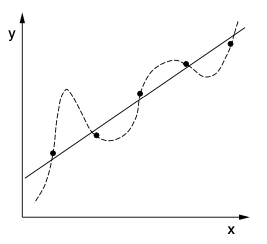
\includegraphics[width=0.5\textwidth]{Images/1.png}
    \caption{Dos posibles modelos de regresión, uno lineal y otro no, para un conjunto de datos dado.}
    \label{fig:Sobreajuste y subajuste}
\end{figure}

¿Pero qué sucede con los riesgos verdaderos \(R(f_{\text{no lineal}})\) y \(R(f_{\text{lineal}})\)? 
El problema es que no podemos calcular estos riesgos a partir de los datos de entrenamiento. 
Además, las funciones \(f_{\text{no lineal}}\) y \(f_{\text{lineal}}\) tienen comportamientos muy diferentes. 
Por ejemplo, si la línea recta \(f_{\text{lineal}}\) fuera la verdadera función subyacente, 
entonces la función discontinua \(f_{\text{no lineal}}\) tendría un riesgo verdadero elevado, 
ya que la “distancia” entre la función verdadera y la estimada es muy grande. 
Lo mismo ocurre en sentido contrario. En ambos casos, el riesgo verdadero sería mucho mayor que el riesgo empírico.


Este ejemplo resalta una decisión importante que debemos tomar: ¿preferimos ajustar los datos de entrenamiento 
con una función relativamente compleja, lo que conduce a un error de entrenamiento muy pequeño, o preferimos 
ajustarlos con una función simple a costa de un error de entrenamiento ligeramente mayor? En el ejemplo 
anterior, un físico que mida estos puntos de datos podría argumentar que no puede ser coincidencia que las mediciones 
estén casi alineadas y preferiría atribuir los residuos a errores de medición en lugar de a un modelo erróneo. Pero, 
¿es posible caracterizar en qué sentido la línea recta es más simple y por qué esto debería implicar que está, de 
alguna manera, más cerca de la verdadera dependencia subyacente? Es decir, nos interesa saber cuál es el 
aumento en el error de entrenamiento que deberíamos estar dispuestos a tolerar para ajustar un modelo más simple.

De una forma u otra, esta cuestión ha ocupado durante mucho tiempo las mentes de los investigadores que estudian 
el problema del aprendizaje. En la estadística clásica, se ha estudiado como el dilema \textit{sesgo-varianza} 
(\textit{bias-variance tradeoff}). Si ajustamos un modelo lineal para cada conjunto de datos que encontramos, 
podríamos pensar que toda dependencia funcional es lineal. Pero no sería por la naturaleza de los procesos que
generan los datos, sino un sesgo impuesto por nosotros. Por otro lado, 
si tomamos un polinomio de grado suficientemente alto para cualquier muestra, siempre podríamos ajustar 
perfectamente los datos, pero el modelo exacto que obtendríamos estaría sujeto a grandes fluctuaciones, dependiendo 
de qué tan precisas fueran nuestras mediciones en primer lugar. Esto implicaría que el modelo sufra de una gran varianza.

Una dicotomía relacionada es la existente entre el error de estimación y el error de aproximación. Si usamos una clase 
pequeña de funciones, incluso la mejor solución posible aproximará pobremente la dependencia real, mientras 
que una clase grande de funciones llevará a un error de estimación estadística alto. En la terminología del aprendizaje 
estádistico aplicado, el modelo complejo muestra \textbf{sobreajuste} (overfitting), 
mientras que el modelo lineal simple es más proclive a sufrir de \textbf{subajuste} (underfitting).

\subsection{Los dilemas sesgo-varianza y estimación-aproximación}


El ejemplo ilustrado en la Figura ~\ref{fig:Sobreajuste y subajuste}
ya señaló de manera intuitiva el problema de la complejidad del modelo: ¿cuándo un modelo es “más simple” que otro? 
¿Es bueno que un modelo sea simple? ¿Qué tan simple? 
Ya hemos mencionado anteriormente que el objetivo de la clasificación es lograr un riesgo tan bueno 
como el del clasificador de Bayes. ¿Podríamos simplemente elegir \(\mathcal{F}\) como el espacio \(\mathcal{F}_{\text{all}}\) 
de todas las funciones, definir el clasificador \(f_n := \arg\min_{f \in \mathcal{F}_{\text{all}}} \left(\mathcal{R}_{\text{emp}}(f)\right)\), 
y obtener consistencia? Desafortunadamente, la respuesta es no. Luego veremos que, 
si optimizamos sobre clases de funciones \(\mathcal{F}\) demasiado grandes, y en particular si hacemos \(\mathcal{F}\) tan 
grande que contenga todos los clasificadores de Bayes para todas las distribuciones de probabilidad \(P\), 
esto conduce a la inconsistencia. Por lo tanto, si queremos aprender con éxito, necesitamos trabajar 
con una clase de funciones \(\mathcal{F}\) más pequeña. Para investigar las propiedades contrapuestas de la 
complejidad del modelo y la generalización, queremos introducir algunas nociones que serán útiles más adelante.

Recordemos las definiciones \(f_n\), \(f_\mathcal{F}\) y \(f_{\text{Bayes}}\) introducidas anteriormente. Hemos visto que 
la consistencia de Bayes trata sobre la convergencia del término \(R(f_n) - R(f_{\text{Bayes}})\). 
Es importante notar que podemos descomponer esta cantidad de la siguiente manera:
\[ 
\mathcal{R}(f_n) - \mathcal{R}(f_{\text{Bayes}}) = \underbrace{\mathcal{R}(f_n) - \mathcal{R}(f_\mathcal{F})}_{\text{error de generalización}} +
\underbrace{\mathcal{R}(f_\mathcal{F}) - \mathcal{R}(f_{\text{Bayes}})}_{\text{error de aproximación}} 
\]

Los dos términos en el lado derecho tienen nombres particulares: el primero se denomina 
\textbf{error de estimación} y el segundo \textbf{error de aproximación}. En la Figura 
\ref{fig:error de estimación y aproximación} 
tenemos una ilustración. El primer término aborda la 
incertidumbre introducida por el proceso de muestreo aleatorio. Dado un conjunto de datos 
finitos, necesitamos estimar la mejor función en \(\mathcal{F}\). Por supuesto, en este proceso cometeremos 
errores. Este error se denomina error de estimación. El segundo término no está influido por cantidades aleatorias.
Trata sobre el error que cometemos al buscar la mejor función en un espacio de funciones \(\mathcal{F}\) pequeño, 
en lugar de buscar la mejor función en el espacio \(F_{\text{all}}\) de todas las funciones posibles. 
La pregunta fundamental en este contexto es qué tan bien las funciones en \(\mathcal{F}\) pueden aproximar a las 
funciones en \(F_{\text{all}}\) y de allí proviene el nombre error de aproximación.

\begin{figure}[h!]
    \centering
    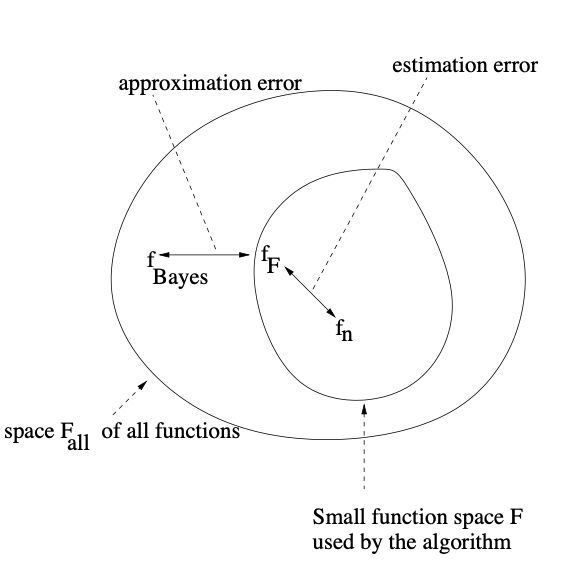
\includegraphics[width=0.5\textwidth]{Images/2.png}
    \caption{Error de estimación y de aproximación.}
    \label{fig:error de estimación y aproximación}
\end{figure}


En estadística, el error de estimación también se llama \textbf{varianza}, y el error de aproximación 
se llama \textbf{sesgo} de un estimador. Originalmente, estos términos se acuñaron para la situación 
especial de regresión con función de pérdida cuadrática, pero ahora se usan en contextos más generales, 
como el que se describe aquí. Su significado intuitivo es el mismo: el primer término mide la 
variación del riesgo de la función \(f_n\) estimada en la muestra, mientras que el segundo mide el 
sesgo introducido en el modelo al elegir una clase de funciones demasiado pequeña.

En este punto, ya podemos señalar que el espacio \(\mathcal{F}\) es el medio para equilibrar el compromiso 
entre el error de estimación y el error de aproximación. Podemos hacernos una idea gráfica viendo la Figura
. Si elegimos un espacio \(\mathcal{F}\) muy grande, el 
término de aproximación será pequeño (el clasificador de Bayes podría incluso estar contenido en 
\(\mathcal{F}\) o ser aproximado de manera cercana por algún elemento en \(\mathcal{F}\)). Sin embargo, el error de 
estimación será bastante grande en este caso: el espacio \(\mathcal{F}\) contendrá funciones complejas que 
conducirán al \textbf{sobreajuste} (overfitting). El efecto opuesto ocurrirá si la clase de funciones 
\(\mathcal{F}\) es muy pequeña.
\begin{figure}[h!]
    \centering
    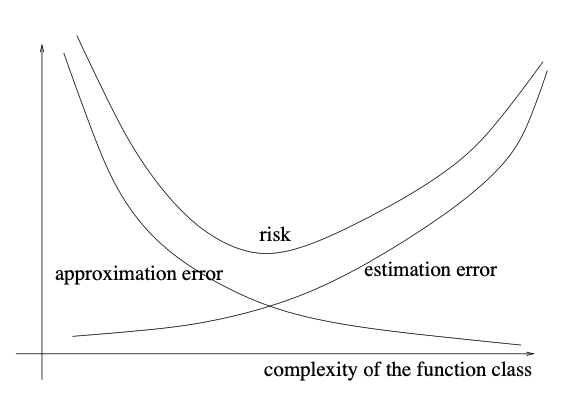
\includegraphics[width=0.5\textwidth]{Images/3.png}
    \caption{Compromiso entre error de estimación y de aproximación. Si el espacio funcional $\mathcal{F}$ que define
    el algoritmo de aprendizaje es pequeño, es decir es poco complejo, el error de estimación es bajo, pero el de aproximación
    es alto, y estamos en una situación proclive al subajuste. Si, por otro lado,  $\mathcal{F}$ es complejo, el error de estimación
    es alto y el de aproximación bajo, y tendemos al sobreajuste. El error ideal es usualmente obtenido con una complejidad moderada.}
    \label{fig:Compromiso entre error de estimación y de aproximación.}
\end{figure}

En lo que sigue, trataremos el error de estimación y el error de aproximación por separado. Veremos 
que tienen comportamientos bastante diferentes y que se necesitan métodos distintos para controlar 
cada uno.

\section{El clasificador de los $k$ vecinos más cercanos}

Hasta 1977, no se sabía si existía un clasificador universalmente consistente. 
Esta pregunta fue resuelta positivamente por Stone (1977), quien demostró, mediante una elegante prueba, 
que un clasificador particular, el denominado clasificador de los \(k\)-vecinos más cercanos 
(\textit{k-nearest neighbors classifier}, abreviado como $k$-NN), es universalmente consistente. Como el clasificador de los \(k\)-vecinos 
más cercanos es uno de los clasificadores más simples y todavía se usa ampliamente en la práctica, 
dedicaremos esta sección a ilustrar las nociones introducidas en la sección anterior, tales como 
generalización, sobreajuste, subajuste y consistencia, usando el ejemplo del clasificador \(k\)-NN.

Consideremos una muestra de puntos con etiquetas \((X_1, Y_1), \dots, (X_n, Y_n)\) que 
pertenecen a un espacio métrico. De manera general, el paradigma del aprendizaje consiste en asignar salidas 
similares a entradas similares. Es decir, creemos que los puntos que están cercanos en el espacio 
de entrada tienden a tener la misma etiqueta en el espacio de salida. Nótese que si esta afirmación 
no se cumple, el aprendizaje se vuelve muy difícil o incluso imposible. Para un aprendizaje exitoso, 
debe existir alguna forma de relacionar las etiquetas de los puntos de entrenamiento con las de los 
puntos de prueba, y esto siempre implica suposiciones previas sobre las relaciones entre los puntos 
de entrada. La relación más simple es una distancia entre puntos, pero existen otras formas de medir 
la similitud, como los \textit{kernels}, que forman la base de algunos de los algoritmos 
de aprendizaje más populares (Schölkopf y Smola, 2002).

Supongamos entonces que existe una función de distancia en el espacio de entrada, es decir, una función 
\(d : X \times X \to \mathbb{R}\), que asigna un valor de distancia \(d(X, X')\) a cada par de puntos 
de entrenamiento \(X, X'\). Dados algunos puntos de entrenamiento, ahora queremos predecir una buena 
etiqueta para un nuevo punto \(X\) que no se halla en el conjunto de entrenamiento.
 Una idea simple es buscar el punto de entrenamiento \(X_i\) 
que tenga la distancia más pequeña a \(X\) y asignar a \(X\) la etiqueta correspondiente \(Y_i\) de 
ese punto. Para definir esto de manera más formal, denotamos por \(\text{NN}(X)\) al vecino más cercano 
de \(X\) entre todos los puntos de entrenamiento, es decir:

\[
\text{NN}(X) = \arg\min \{X' \in \{X_1, \dots, X_n\} \mid d(X, X') \leq d(X, X'') \ \text{para todo} \ X'' \in \{X_1, \dots, X_n\}\}.
\]

Luego, podemos definir el clasificador \(f_n\) basado en la muestra de \(n\) puntos como:

\[
f_n(X) = Y_i \quad \text{donde} \quad X_i = \text{NN}(X).
\]

Este clasificador se denomina clasificador de un vecino más cercano (\textit{1-nearest neighbor}, 1NN). 
Podemos generalizarlo en el clasificador de los \(k\)-vecinos más cercanos (\textit{kNN}), considerando los \(k\) puntos de 
entrenamiento más cercanos, con $k>1$ en este caso, y tomando el promedio de todas sus etiquetas. 


\begin{dfn}
    Dados un espacio métrico \(X\) junto a una función de distancia \(d : X \times X \to \mathbb{R}\), 
    un conjunto de puntos de entrenamiento con sus etiquetas \((X_1, Y_1), \dots, (X_n, Y_n)\) y un entero \(k \geq 1\), 
    definimos los \textbf{\(k\)-vecinos más cercanos} de un punto \(X\) como el conjunto de los \(k\) puntos 
    de entrenamiento más cercanos a \(X\), es decir:

    \[
    \text{kNN}(X) = \{X_{i_1}, \dots, X_{i_k}\} \quad \text{donde} \quad i_1, \dots, i_k = \arg\min_{1 \leq j \leq n} d(X, X_j).
    \]
\end{dfn}

Es decir, definimos los 
\(k\)-vecinos más cercanos de \(X\), \(\text{kNN}(X)\), como el conjunto de los \(k\) puntos de 
entrenamiento más cercanos a \(X\). Luego, el clasificador \(k\)-NN se define como:

\begin{dfn}
    Con las mismas condiciones de la definición anterior,
    definimos el \textbf{clasificador de los \(k\)-vecinos más cercanos} como la función \(f_n : X \to Y\) 
    que asigna a un punto \(X\) la etiqueta que resulta de una votación mayoritaria entre las etiquetas 
    de los puntos de entrenamiento en la vecindad de \(k\)-vecinos más cercanos de \(X\):


    \[
f_n(X) = 
\begin{cases} 
+1 & \text{si } \sum_{X_i \in \text{kNN}(X)} Y_i > 0, \\ 
-1 & \text{en otro caso}.
\end{cases}
\]
\end{dfn}


Es decir, decidimos la etiqueta de \(X\) mediante una votación mayoritaria entre las etiquetas de los 
puntos de entrenamiento en la vecindad de \(k\)-vecinos más cercanos de \(X\). Para evitar empates, 
generalmente se elige \(k\) como un número impar.


\begin{thm}
    El clasificador de un vecino más cercano (1NN) no es Bayes-consistente.
\end{thm}

\begin{proof}

Consideremos 
el intervalo real \(X = [0, 1]\) y la distribución de probabilidad \(P([0, 1])\),  que asigna etiquetas 
de manera uniforme a todos los puntos \(X \in [0, 1]\) con ruido, de modo que 
\(P(Y = 1 \mid X = x) = 0.9\) para todo \(x \in X\). Es decir, la etiqueta correcta (la que 
asigna el clasificador de Bayes) es \(+1\) para todos los puntos \(x \in X\). Ya hemos mencionado 
este ejemplo cuando introdujimos el clasificador de Bayes. En este caso, el clasificador de Bayes 
es simplemente la función que devuelve \(1\) para todos los puntos en \(X\), y su riesgo Bayesiano 
con respecto a la pérdida 0-1 será

\[
\begin{aligned}
    \mathcal{R}(f_{\text{Bayes}}) & = \mathbb{E}(\ell(X,Y,f_{\text{Bayes}}(X))) \\
    & = \mathbb{E}(1\cdot P(f_{\text{Bayes}}(X)\neq Y) + 0 \cdot P(f_{\text{Bayes}}(X) = Y))\\
    & = \mathbb{E}(P(f_{\text{Bayes}}(X)\neq Y))\\
    & = \int_{0}^{1} P(Y = 1 \mid X = x) \cdot \mathbb{I}_{\{f_{\text{Bayes}}(x) \neq 1\}} \, dx \\
    & \qquad \qquad + \int_{0}^{1} P(Y=0 \mid X=x) \cdot \mathbb{I}_{\{f_{\text{Bayes}}(x) = 1\}} \\
    & = \int_{0}^{1} (0.9 \cdot 0 + 0.1 \cdot 1) \, dx = 0.1.
\end{aligned}
\]

Ahora investiguemos el comportamiento del clasificador 1NN 
en este caso. Al tomar puntos de entrenamiento \((X_i, Y_i)_{i=1,\dots,n}\) de acuerdo con la 
distribución subyacente, estos estarán aproximadamente uniformemente distribuidos en el intervalo 
\([0, 1]\). En promedio, cada décimo punto tendrá una etiqueta de entrenamiento \(Y = -1\), y todos 
los demás tendrán etiqueta \(Y = +1\). Si ahora consideramos el comportamiento del clasificador \(f_n\), 
podemos escribir la probabilidad de que el clasificador 1NN cometa un error al etiqueta un punto como:

\[
\begin{aligned}
P(Y \neq f_n(X)) & = P(Y = 1 \mid f_n(X) = 0) + P(Y = 0 \mid f_n(X) = 1) \\
                 & = 0.1 \cdot 0.9 + 0.9 \cdot 0.1 \\
                 & = 2 \cdot 0.1 \cdot 0.9 = 0.18.
\end{aligned}
\]

Podemos ver que el riesgo \(R(f_n)\) del clasificador \(f_n\) es también $0,18$,
independientemente del tamaño de la muestra $n$. En efecto:

\[
\begin{aligned}
    \mathcal{R}(f_n) & = \mathbb{E}(\ell(X,Y,f_n(X))) \\
    & = \int_{0}^{1} 1\cdot P(Y \neq f_n(X=x)) + 0 \cdot P(Y = f_n(X=x)) \, dx \\
    & = \int_{0}^{1} P(Y \neq f_n(X=x)) \, dx \\
    & = \int_{0}^{1} 0.18 \, dx = 0.18.
\end{aligned}
\]

Por otro lado el riesgo Bayesiano es $0.1$. Por lo tanto, el clasificador $1$NN no es consistente, ya que 
\(R(f_n) \not\to R(f_{\text{Bayes}})\).
\end{proof}

Consideremos por un momento el clasificador de los 100 vecinos 
más cercanos, $100$NN. En este caso, el clasificador cometería muchos menos errores que su primo de un vecino: 
es muy poco probable tener una vecindad de 100 puntos donde la mayoría de los votos sean \(Y = -1\). 
Así, el clasificador de 100 vecinos más cercanos, aunque sigue sin ser consistente, comete un error 
menor que el clasificador 1NN.

El truco para lograr consistencia está relacionado con esta observación. Esencialmente, se debe permitir 
que el tamaño \(k\) de la vecindad bajo consideración crezca con el tamaño de la muestra \(n\). Formalmente, 
se puede demostrar el siguiente teorema:


\begin{thm}[Stone, 1977]
Sea \(f_n\) el clasificador de los \(k\)-vecinos más cercanos construido 
a partir de una muestra de \(n\) puntos. Si \(n \to \infty\) y \(k \to \infty\) de modo que \(k/n \to 0\), 
entonces \(R(f_n) \to R(f_{\text{Bayes}})\) para todas las distribuciones de probabilidad \(P\). 
Es decir, la regla de clasificación \(k\)-NN es universalmente consistente con Bayes.
\end{thm}

Este teorema esencialmente nos dice que si elegimos el parámetro de vecindad \(k\) de forma que crezca 
lentamente con \(n\), por ejemplo \(k \approx \log(n)\), entonces la regla de clasificación \(k\)-NN es 
universalmente Bayes-consistente.

En las secciones anteriores mencionamos que la clase de funciones \(\mathcal{F}\) de la cual se elige el clasificador 
es un componente importante para la teoría del aprendizaje estadístico. En el caso del clasificador \(k\)-NN, 
esto no es tan obvio como lo será para los clasificadores que estudiaremos en secciones posteriores. 
Intuitivamente, se puede decir que, para un parámetro fijo \(k\), la clase de funciones \(\mathcal{F}_k\) es un espacio 
de funciones constantes por partes. Cuanto mayor sea \(k\), más grandes serán las vecindades de los \(k\)-vecinos 
y, por lo tanto, mayores serán los segmentos donde las funciones deben ser constantes. Esto significa que, 
para valores muy grandes de \(k\), la clase de funciones \(\mathcal{F}_k\) es relativamente pequeña (las funciones no 
pueden oscilar mucho). En el caso extremo de \(k = n\), la vecindad de los \(k\)-vecinos simplemente incluye 
todos los puntos de entrenamiento, por lo que el clasificador \(k\)-NN no puede cambiar su signo en absoluto; 
debe ser constante en todo el espacio de entrada \(X\). En este caso, la clase de funciones \(\mathcal{F}_k\) contiene solo 
dos elementos: la función que es constantemente \(+1\) y la función que es constantemente \(-1\).

Por otro lado, si \(k\) es pequeño, entonces \(\mathcal{F}_k\) se vuelve bastante grande (las funciones pueden cambiar sus 
etiquetas con mucha frecuencia y de manera abrupta). En los términos explicados en las secciones anteriores, 
podemos decir que si elegimos \(k\) demasiado pequeño, entonces la clase de funciones sobreajusta; 
por ejemplo, esto ocurre en el caso extremo del clasificador 1NN. Por el contrario, si \(k\) es demasiado grande, 
la clase de funciones subajusta, ya que simplemente no contiene funciones capaces de modelar los 
datos de entrenamiento.

\section{Minimización del riesgo empírico}

En la sección anterior encontramos nuestro primer clasificador simple: el clasificador \(k\)-NN. En esta sección, 
queremos abordar una forma más poderosa de clasificar datos, el llamado principio de \textbf{minimización 
del riesgo empírico}. Recordemos la suposición de que los datos son generados de manera \textit{iid} 
(independientes e idénticamente distribuidos) a partir de una distribución subyacente desconocida \(P(X, Y)\). 
Como ya hemos visto, el problema de aprendizaje consiste en minimizar el riesgo (o pérdida esperada sobre 
los datos de prueba):

\[
\mathcal{R}(f) = \mathbb{E}(\ell(X, Y, f(X))),
\]

donde \(f\) es una función que mapea el espacio de entrada \(X\) al espacio de etiquetas \(Y\), y \(\ell\) 
es la función de pérdida. 

La dificultad de esta tarea radica en el hecho de que estamos intentando minimizar una cantidad que no 
podemos evaluar directamente: dado que no conocemos la distribución de probabilidad subyacente \(P\), 
no podemos calcular el riesgo \(\mathcal{R}(f)\). Sin embargo, lo que sí conocemos son los datos de entrenamiento, 
muestreados a partir de \(P\). Por lo tanto, podemos intentar inferir una función \(f\) a partir de la muestra 
de entrenamiento cuyo riesgo esté cercano al mejor riesgo posible. Para ello, necesitamos lo que se llama 
un \textit{principio de inducción}.

Quizás la forma más directa de proceder sea aproximar el riesgo verdadero mediante el \textbf{riesgo empírico} 
calculado sobre los datos de entrenamiento. En lugar de buscar una función que minimice el riesgo verdadero 
\(\mathcal{R}(f)\), intentamos encontrar aquella que minimice el riesgo empírico:

\[
\mathcal{R}_{\text{emp}}(f) = \frac{1}{n} \sum_{i=1}^{n} \ell(X_i, Y_i, f(X_i)).
\]

Es decir, dados algunos datos de entrenamiento \((X_1, Y_1), \dots, (X_n, Y_n)\), un espacio de funciones 
\(F\) con el cual trabajar, y una función de pérdida \(\ell\), definimos el clasificador \(f_n\) como la función:

\[
f_n := \arg\min_{f \in \mathcal{F}} \mathcal{R}_{\text{emp}}(f).
\]

Este enfoque se denomina \textbf{principio de inducción de minimización del riesgo empírico}, abreviado como 
ERM (\textit{Empirical Risk Minimization}). La motivación para este principio está dada por la ley de los 
grandes números, como explicaremos a continuación.

\subsection{La ley de los grandes números}

Recordemos que, en su forma más simple, la ley de los grandes números
establece que, bajo condiciones suaves, la media de variables aleatorias \(\xi_i\) que han sido extraídas 
de manera \textit{iid} (independiente e idénticamente distribuida) a partir de una distribución de probabilidad 
\(P\), converge a la media de la distribución subyacente cuando el tamaño de la muestra tiende a infinito:

\[
\frac{1}{n} \sum_{i=1}^n \xi_i \to \mathbb{E}(\xi) \quad \text{cuando } n \to \infty.
\]

Aquí, la notación supone que la secuencia \(\xi_1, \xi_2, \dots\) ha sido muestreada de manera \textit{iid} 
a partir de \(P\) y que \(\xi\) también está distribuida según \(P\). Este teorema puede aplicarse al caso del 
riesgo empírico y el riesgo verdadero. Para ver esto, notemos que el riesgo empírico se define como la media de 
la pérdida \(\ell(X_i, Y_i, f(X_i))\) en puntos de muestra individuales, y el riesgo verdadero es la media de 
esta pérdida sobre toda la distribución. Es decir, a partir de la ley de los grandes números, podemos concluir 
que, para una función fija \(f\), el riesgo empírico converge al riesgo verdadero a medida que el tamaño de la 
muestra tiende a infinito:

\[
\mathcal{R}_{\text{emp}}(f) = \frac{1}{n} \sum_{i=1}^n \ell(X_i, Y_i, f(X_i)) \to \mathbb{E}(\ell(X, Y, f(X))) \quad 
\text{cuando } n \to \infty.
\]

Aquí, la función de pérdida \(\ell(X, Y, f(X))\) desempeña el papel de la variable aleatoria \(\xi\). Para una 
muestra finita dada, esto significa que podemos aproximar el riesgo verdadero (el que nos interesa) de manera 
bastante precisa mediante el riesgo empírico (el que podemos calcular sobre la muestra).

Una desigualdad famosa, atribuida a Chernoff (1952) y luego generalizada por Hoeffding (1963), caracteriza qué 
tan bien la media empírica aproxima el valor esperado. Específicamente, si las variables aleatorias \(\xi_i\) 
toman valores solo en el intervalo \([0, 1]\), entonces:

\begin{equation}
P\left( \left| \frac{1}{n} \sum_{i=1}^n \xi_i - \mathbb{E}(\xi) \right| \geq \epsilon \right) \leq 
2 \exp(-2n\epsilon^2). 
\end{equation}

Este teorema establece que la probabilidad de que la media de la muestra se desvíe más de \(\epsilon\) del 
valor esperado de la distribución está acotada por una cantidad muy pequeña, específicamente \(2 \exp(-2n\epsilon^2)\). 
Nótese que, cuanto mayor sea \(n\), más pequeña será esta cantidad; es decir, la probabilidad de desviaciones 
grandes disminuye rápidamente con \(n\). Una vez más, podemos aplicar este teorema al contexto del riesgo empírico 
y verdadero. Esto conduce a una cota que establece qué tan probable es que el riesgo empírico esté cerca del 
riesgo verdadero para una función dada \(f\):

\begin{equation}
P(|\mathcal{R}_{\text{emp}}(f) - \mathcal{R}(f)| \geq \epsilon) \leq 2 \exp(-2n\epsilon^2).  \label{eq:Chernoff}
\end{equation}

Para cualquier función fija (y un \(n\) suficientemente grande), es muy probable que el error de entrenamiento 
proporcione una buena estimación del error de prueba.

Existen algunos hechos importantes relacionados con la cota de Chernoff (\ref{eq:Chernoff}). Primero, una propiedad crucial 
de la cota de Chernoff es que es de naturaleza probabilística. Establece que la probabilidad de una gran desviación 
entre el error de prueba y el error de entrenamiento de \(f\) es pequeña; cuanto mayor sea el tamaño de la muestra 
\(n\), menor será esta probabilidad. Por lo tanto, no descarta la presencia de casos en los que la desviación sea 
grande; simplemente dice que, para una función fija \(f\), esto es muy poco probable. La razón de esto radica en la 
generación aleatoria de los puntos de entrenamiento. Podría ocurrir que, en algunos casos desafortunados, nuestros 
datos de entrenamiento sean tan engañosos que sea imposible construir un buen clasificador a partir de ellos. Sin 
embargo, a medida que el tamaño de la muestra aumenta, tales casos desafortunados se vuelven muy raros. En este 
sentido, cualquier garantía de consistencia solo puede ser de la forma: el riesgo empírico está cerca del riesgo 
verdadero, con alta probabilidad.

A primera vista, parece que la cota de Chernoff (\ref{eq:Chernoff}) es suficiente para probar la consistencia de la minimización 
del riesgo empírico. Sin embargo, hay una advertencia importante: la cota de Chernoff solo se cumple para una función 
fija \(f\) que no depende de los datos de entrenamiento. Sin embargo, el clasificador \(f_n\), por supuesto, depende 
de los datos de entrenamiento (usamos los datos de entrenamiento para seleccionar \(f_n\)). Aunque esto pueda parecer 
una diferencia matemática sutil, aquí es donde la minimización del riesgo empírico puede fallar por completo. A 
continuación, discutiremos este problema en detalle y veremos cómo adaptar la ley fuerte de los grandes números para 
poder tratar funciones que dependen de los datos.

\subsection{Inconsistencia en la minimización del riesgo empírico} \label{Inconsistencia en la minimización del riesgo empírico}

Supongamos que nuestro espacio de datos subyacente es \(X = [0,1]\). Elegimos la distribución uniforme sobre 
\(X\) como la distribución de probabilidad y definimos la etiqueta \(Y\) para un punto de entrada \(X\) de 
manera determinista como sigue:

\[
Y = 
\begin{cases} 
-1 & \text{si } X < 0.5, \\ 
1 & \text{si } X \geq 0.5.
\end{cases}
\]

Ahora supongamos que se nos da un conjunto de puntos de entrenamiento \((X_i, Y_i)_{i=1,\dots,n}\) y 
consideremos el siguiente clasificador:

\[
f_n(X) = 
\begin{cases} 
Y_i & \text{si } X = X_i \text{ para algún } i = 1, \dots, n, \\ 
1 & \text{en otro caso.}
\end{cases}
\]

Este clasificador \(f_n\) clasifica perfectamente todos los puntos de entrenamiento. Es decir, tiene un 
riesgo empírico \(\mathcal{R}_{\text{emp}}(f_n) = 0\). En consecuencia, dado que el riesgo empírico no puede ser 
negativo, \(f_n\) es un minimizador del riesgo empírico. Sin embargo, \(f_n\) claramente no ha aprendido 
nada; el clasificador simplemente memoriza las etiquetas de entrenamiento y, en otros casos, predice 
simplemente la etiqueta \(1\).

Formalmente, esto significa que el clasificador \(f_n\) no será consistente. Para ver esto, supongamos que 
se nos da un punto de prueba \((X, Y)\) extraído de la distribución subyacente. Usualmente, este punto de 
prueba no será idéntico a ninguno de los puntos de entrenamiento, y en este caso el clasificador simplemente 
predice la etiqueta \(1\). Si \(X\) resulta ser mayor que \(0.5\), esta es la etiqueta correcta, pero si 
\(X < 0.5\), es la etiqueta incorrecta. Por lo tanto, el clasificador \(f_n\) cometerá errores en la mitad 
de todos los puntos de prueba, lo que implica que su error de prueba es \(R(f_n) = 1/2\). Este es el mismo 
error que se obtendría con una predicción aleatoria. De hecho, este es un buen ejemplo de 
\textbf{sobreajuste}: el clasificador \(f_n\) se ajusta perfectamente a los datos de entrenamiento, pero no 
aprende nada sobre los nuevos datos de prueba.

Es fácil ver que el clasificador \(f_n\) es inconsistente. Nótese que, como las etiquetas son una función 
determinista de los puntos de entrada, el clasificador de Bayes tiene un riesgo igual a \(0\). Así, tenemos:

\[
\frac{1}{2} = R(f_n) \not\to R(f_{\text{Bayes}}) = 0.
\]

Hemos construido un ejemplo donde la minimización del riesgo empírico falla de manera estrepitosa. ¿Existe 
alguna manera de rescatar el principio de ERM? Afortunadamente, la respuesta es sí. El objeto principal al 
que debemos prestar atención es la clase de funciones \(\mathcal{F}\) de la cual extraemos nuestro clasificador. Si 
permitimos que nuestra clase de funciones contenga funciones que simplemente memorizan los datos de 
entrenamiento, entonces el principio de ERM no puede funcionar. En particular, si elegimos el minimizador 
del riesgo empírico del espacio \(F_{\text{all}}\) de todas las funciones entre \(X\) e \(Y\), entonces los 
valores de \(f_n\) en los puntos de entrenamiento \(X_1, \dots, X_n\) no necesariamente contienen ninguna 
información sobre los valores en otros puntos. Por lo tanto, a menos que impongamos restricciones en el 
espacio de funciones del cual elegimos nuestra estimación \(f\), no podemos esperar aprender nada. 


\subsection{Convergencia uniforme}

Resulta que las condiciones necesarias para que la minimización del riesgo empírico sea consistente 
implican restringir el conjunto de funciones admisibles. La idea principal de la teoría de Vapnik-Chervonenkis 
(VC) es que la consistencia de la minimización del riesgo empírico está determinada por el comportamiento 
en el peor caso sobre todas las funciones \(f \in \mathcal{F}\) que la máquina de aprendizaje podría elegir. Veremos que, 
en lugar de la ley estándar de los grandes números introducida anteriormente, este caso extremo corresponde 
a una versión de la ley de los grandes números que es uniforme sobre todas las funciones en \(\mathcal{F}\).

\begin{figure}[h]
    \centering
    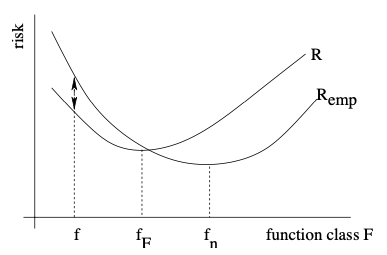
\includegraphics[width=0.8\textwidth]{Images/4.png}
    
    \caption{Representación simplificada de la convergencia del riesgo empírico al riesgo verdadero. El eje \(x\) 
    representa una dimensión de la clase de funciones \(F\), mientras que el eje \(y\) denota el riesgo. Para cada 
    función fija \(f\), la ley de los grandes números nos dice que, a medida que el tamaño de la muestra tiende a 
    infinito, el riesgo empírico \(\mathcal{R}_{\text{emp}}(f)\) converge al riesgo verdadero \(\mathcal{R}(f)\) (indicado por la flecha). 
    Sin embargo, esto no implica que, en el límite de tamaños de muestra infinitos, el minimizador del riesgo 
    empírico, \(f_n\), lleve a un valor del riesgo tan bueno como el del mejor \(f_F\) en la clase de funciones. 
    Para que esto sea cierto, requerimos la convergencia uniforme de \(\mathcal{R}_{\text{emp}}(f)\) a \(\mathcal{R}(f)\) sobre todas 
    las funciones en \(F\). (Adaptado de Schölkopf y Smola, 2002).}
    \label{riesgo vs riesgo empirico}
    \end{figure}
    
La Figura \ref{riesgo vs riesgo empirico} presenta una representación simplificada de la ley uniforme de los grandes números y la cuestión 
de la consistencia. Tanto el riesgo empírico como el riesgo verdadero se grafican como funciones de \(f\). 
Para simplificar, hemos resumido todas las funciones posibles \(f\) en un solo eje del gráfico. La minimización 
del riesgo empírico consiste en elegir la función \(f\) que minimiza \(\mathcal{R}_{\text{emp}}\). Es consistente si el 
mínimo de \(\mathcal{R}_{\text{emp}}\) converge al de \(R\) a medida que el tamaño de la muestra aumenta. Una forma de 
garantizar la convergencia del mínimo para todas las funciones en \(\mathcal{F}\) es la \textbf{convergencia uniforme} sobre 
\(\mathcal{F}\): requerimos que para todas las funciones \(f \in \mathcal{F}\), la diferencia entre \(\mathcal{R}(f)\) y \(\mathcal{R}_{\text{emp}}(f)\) 
se vuelva pequeña simultáneamente. Es decir, requerimos que exista un valor grande de \(n\) tal que, para un 
tamaño de muestra al menos \(n\):

\[
\sup_{f \in \mathcal{F}} |\mathcal{R}(f) - \mathcal{R}_{\text{emp}}(f)| \leq \epsilon.
\]

Luego

\[
|\mathcal{R}(f) - \mathcal{R}_{\text{emp}}(f)| \leq \sup_{f \in \mathcal{F}} |\mathcal{R}(f) - \mathcal{R}_{\text{emp}}(f)|.
\]

En particular, esto también se cumple para una función \(f_n\) que se haya elegido en base a una muestra finita 
de puntos de entrenamiento

\begin{equation}
P(|R(f_n) - \mathcal{R}_{\text{emp}}(f_n)| \geq \epsilon) \leq P\left(\sup_{f \in \mathcal{F}} |\mathcal{R}(f) - \mathcal{R}_{\text{emp}}(f)| \geq \epsilon\right). \label{eq:cota_uniforme}
\end{equation}

La cantidad en el lado derecho de la ecuación (\ref{eq:cota_uniforme}) es ahora el objeto de la ley uniforme de los grandes números. 
Decimos que la ley de los grandes números se cumple de manera uniforme sobre una clase de funciones \(\mathcal{F}\) si, 
para todo \(\epsilon > 0\),

\[
P\left(\sup_{f \in \mathcal{F}} |\mathcal{R}(f) - \mathcal{R}_{\text{emp}}(f)| \geq \epsilon \right) \to 0 \quad \text{cuando } n \to \infty.
\]

Ahora podemos usar la ecuación (\ref{eq:cota_uniforme}) para mostrar que, si la ley uniforme de los grandes números se cumple para 
alguna clase de funciones \(\mathcal{F}\), entonces la minimización del riesgo empírico es consistente con respecto a \(\mathcal{F}\). 
Para verlo, consideremos:

\[
|R(f_n) - R(f_\mathcal{F})| = R(f_n) - R(f_\mathcal{F})
\]

Puesto que  \(R(f_n) - R(f_\mathcal{F}) \geq 0\), por definición de \(f_\mathcal{F}\). Sumando y restando cantidades idénticas,
esta expresión se puede reescribir como:
\[
R(f_n) - \mathcal{R}_{\text{emp}}(f_n) + \mathcal{R}_{\text{emp}}(f_n) - \mathcal{R}_{\text{emp}}(f_\mathcal{F}) + \mathcal{R}_{\text{emp}}(f_F) - R(f_\mathcal{F})
\]
\[
    \leq R(f_n) - \mathcal{R}_{\text{emp}}(f_n) + \mathcal{R}_{\text{emp}}(f_\mathcal{F}) - R(f_\mathcal{F})
\] 
\[
    \leq 2 \sup_{f \in \mathcal{F}} |\mathcal{R}(f) - \mathcal{R}_{\text{emp}}(f)|.
\]
Dado que \(\mathcal{R}_{\text{emp}}(f_n) - \mathcal{R}_{\text{emp}}(f_\mathcal{F}) \leq 0\) por definición de \(f_n\), y luego acotando
al tomar el supremo de todas las funciones en el espacio $\mathcal{F}$.\\

De esto podemos concluir:

\[
P\left(|R(f_n) - R(f_\mathcal{F})| \geq \epsilon \right) \leq P\left(\sup_{f \in \mathcal{F}} |\mathcal{R}(f) - \mathcal{R}_{\text{emp}}(f)| \geq \epsilon/2\right).
\]

Bajo la ley uniforme de los grandes números, el lado derecho tiende a \(0\), lo que lleva a la consistencia de 
la minimización del riesgo empírico con respecto a la clase de funciones subyacente \(\mathcal{F}\). En otras palabras, 
la convergencia uniforme sobre \(\mathcal{F}\) es una condición suficiente para la consistencia de la minimización del 
riesgo empírico sobre \(\mathcal{F}\).


Parte de la elegancia de la teoría VC radica en que el recíproco también es cierto. Es decir, 
la convergencia uniforme no solo es una condición suficiente, sino también una condición necesaria para la 
consistencia de la minimización del riesgo empírico con respecto a \(\mathcal{F}\). Esto se formaliza en el siguiente 
teorema:

\begin{thm}[Vapnik y Chervonenkis, 1971]
La convergencia uniforme
    
    \[
        P\left(\sup_{f \in \mathcal{F}} |\mathcal{R}(f) - \mathcal{R}_{\text{emp}}(f)| > \epsilon \right) \to 0 \quad \text{cuando } n \to \infty, 
        \]
        
        para todo \(\epsilon > 0\), es una condición necesaria y suficiente para la consistencia de la minimización del 
        riesgo empírico con respecto a \(\mathcal{F}\).
\end{thm}
        
En la sección \ref{Inconsistencia en la minimización del riesgo empírico} dimos un ejemplo donde consideramos el conjunto de todas las funciones posibles y mostramos 
que el aprendizaje era imposible. Ahora, la dependencia del aprendizaje en el conjunto de funciones subyacente 
ha regresado bajo una forma diferente: la condición de convergencia uniforme depende críticamente del conjunto 
de funciones para el cual debe cumplirse. 

Intuitivamente, parece claro que cuanto mayor sea el espacio de funciones \(\mathcal{F}\), mayor será:

\[
\sup_{f \in \mathcal{F}} |\mathcal{R}(f) - \mathcal{R}_{\text{emp}}(f)|.
\]

Por lo tanto, cuanto mayor sea \(\mathcal{F}\), mayor será la medida de probabilidad:

\[
P\left(\sup_{f \in \mathcal{F}} |\mathcal{R}(f) - \mathcal{R}_{\text{emp}}(f)| > \epsilon \right).
\]

En consecuencia, cuanto mayor sea \(\mathcal{F}\), más difícil será satisfacer la ley uniforme de los grandes números. 
Esto implica que para espacios de funciones más grandes, la consistencia es más difícil de lograr en comparación 
con espacios de funciones más pequeños.


Esta caracterización abstracta de la consistencia como una propiedad de convergencia uniforme es teóricamente 
fascinante, pero no siempre es útil en la práctica. La razón es que parece complicado determinar si la ley uniforme 
de los grandes números se cumple para una clase de funciones \(\mathcal{F}\) particular. Por esta razón, se han desarrollado 
herramientas como la dimensión VC para analizar y limitar la capacidad de las clases de funciones, lo cual discutiremos 
en las siguientes secciones.

\section{Cotas de generalización y medidas de capacidad}

Para hacer afirmaciones sobre lo que ocurre después de observar solo un número finito de puntos de datos 
—que en la práctica será siempre el caso—, necesitamos examinar más de cerca la 
convergencia uniforme del riesgo empírico al verdadero.
 Resultará que esto nos proporcionará cotas sobre el riesgo y también nos dará información sobre 
qué propiedades de las clases de funciones determinan si la convergencia uniforme puede tener lugar. Detengámonos
en la probabilidad del Teorema anterior:

\begin{equation}
P\left(\sup_{f \in \mathcal{F}} |\mathcal{R}(f) - \mathcal{R}_{\text{emp}}(f)| > \epsilon \right). \label{eq:med_unif_riesgo_riesgo_emp}
\end{equation}

Consideremos entonces un espacio de funciones finito, como el que nos encontramos en la práctica. Sea
\(\mathcal{F}_{emp} = \{f_1, f_2, \dots, f_m\}\) un conjunto de \(m\) funciones. Cada una de las funciones 
\(f_i \in \mathcal{F}_{emp}\) satisface la ley estándar de los grandes números en la forma de la cota de Chernoff:

\[
P\left(|R(f_i) - \mathcal{R}_{\text{emp}}(f_i)| \geq \epsilon \right) \leq 2 \exp(-2n\epsilon^2).
\]

Ahora queremos transformar estas afirmaciones sobre funciones individuales \(f_i\) en una ley uniforme de los 
grandes números. Dada la subatividad de la probabilidad, tenemos:

\[
P\left(\sup_{f \in \mathcal{F}} |\mathcal{R}(f) - \mathcal{R}_{\text{emp}}(f)| \geq \epsilon \right) \leq \sum_{i=1}^m P\left(|R(f_i) - \mathcal{R}_{\text{emp}}(f_i)| \geq \epsilon \right).
\]

Y aplicando la cota de Chernoff a cada término en la suma, obtenemos:

\begin{equation}
P\left(\sup_{f \in \mathcal{F}} |\mathcal{R}(f) - \mathcal{R}_{\text{emp}}(f)| \geq \epsilon \right) \leq 2m \exp(-2n\epsilon^2). \label{eq: chernoff acotada por m}
\end{equation}

Si el espacio de funciones \(\mathcal{F}_{emp}\) es fijo, \(m\) puede considerarse una 
constante, y el término \(2m \exp(-2n\epsilon^2)\) converge a \(0\) cuando \(n \to \infty\). Por lo tanto,
la minimización del riesgo empírico sobre un conjunto finito de funciones es consistente con respecto 
a \(\mathcal{F}_{emp}\). \\

En la práctica, nuestros espacios de funciones estarán definidos por los paramétros que nos permitimos 
seleccionar para cada posible clasificador, como la ordenada al origen y la pendiente en el caso de la regresión lineal y serán usualmente
, como en ese ejemplo,
espacios infinitos. Luego veremos que podemos llegar a una desigualdad similar a esta última, reemplazando $m$ por un valor que depende
de cada tipo de espacio funcional y que, de ser finito, será necesariamente polinómico, lo que nos permitirá obtener cotas de generalización.
Llamaremos a dicha cantidad, la \textit{dimensión VC}.

\subsection{Simetrización}

La \textit{simetrización} es un paso técnico importante para usar medidas de capacidad en espacios infinitos de 
funciones. Su propósito principal es reemplazar el evento 

\[
\sup_{f \in \mathcal{F}} |\mathcal{R}(f) - \mathcal{R}_{\text{emp}}(f)|
\]

por un evento alternativo que pueda calcularse únicamente en una muestra dada. Supongamos que tenemos una muestra 
\((X_i, Y_i)_{i=1,\dots,n}\). Ahora introducimos una nueva muestra llamada \textit{muestra fantasma}. 
Esta es simplemente otra muestra \((X'_i, Y'_i)_{i=1,\dots,n}\), que también se extrae de manera 
\textit{iid} de la misma distribución subyacente y que es independiente de la primera muestra. No necesitamos generar 
esta muestra en la práctica; es solo una herramienta matemática para realizar el análisis. 

Dfinimos el riesgo empírico con respecto a esta muestra como \(\mathcal{R}'_{\text{emp}}(f)\). 
Con la ayuda de esta muestra fantasma, podemos demostrar el siguiente resultado:

\begin{thm}[Lema de simetrización]

Sea $m\epsilon^2 \geq 2$. Sea $\mathcal{F}$ el espacio de funciones definido por un algoritmo de aprendizaje. Sean
$(X_i,Y_i)_{i=1,\dots, n}$, $(X_i',Y_i')_{i=1,\dots, n}$ muestras aleatorias iid. Dada $f \in\mathcal{F}$,
sean $\mathcal{R}(f)$ su riesgo, $\mathcal{R}_{emp}(f)$ su riesgo empírico sobre la primera muestra y 
$\mathcal{R}'_{emp}(f)$ el riesgo sobre la segunda. Entonces, para cualquier $\epsilon > 0$

\[
P\left(\sup_{f \in \mathcal{F}} |\mathcal{R}(f) - \mathcal{R}_{\text{emp}}(f)| > 
\epsilon \right) \leq 2P\left(\sup_{f \in \mathcal{F}} |\mathcal{R}_{\text{emp}}(f) - \mathcal{R}'_{\text{emp}}(f)| > \frac{\epsilon}{2}\right).
\]
\end{thm}

Esta desigualdad, nos permite acotar el comportamiento 
de la diferencia \(\mathcal{R}(f) - \mathcal{R}_{\text{emp}}(f)\) mediante la diferencia entre riesgos empíricos \(\mathcal{R}_{\text{emp}}(f)\) y 
\(\mathcal{R}'_{\text{emp}}(f)\) calculados sobre las muestras original y fantasma, respectivamente. Esto nos permite trabajar 
con eventos que depende únicamente de las muestras observadas.\\

Notemos que, incluso si \(\mathcal{F}\) contiene un número infinito de funciones, 
las diferentes formas en que estas pueden clasificar un conjunto de entrenamiento de \(n\) puntos de muestra 
es finita. En efecto, para cualquier punto de entrenamiento dado en la muestra, una función puede tomar solo los valores 
\(-1\) o \(+1\). En una muestra de \(n\) puntos \(\{X_1, \dots, X_n\}\), una función puede actuar de, como 
máximo, \(2^n\) formas diferentes: puede asignar a cada \(Y_i\) el valor \(-1\) o \(+1\). Esto tiene una 
consecuencia muy importante. Incluso si una clase de funciones \(\mathcal{F}\) contiene infinitas funciones, hay como 
mucho \(2^n\) formas diferentes en que esas funciones pueden clasificar los puntos de una muestra finita de 
\(n\) puntos. Tomando

\[
\sup_{f \in \mathcal{F}} |R_{\text{emp}}(f) - R'_{\text{emp}}(f)|,
\]
entonces el supremo efectivamente solo recorre una clase de funciones finita. Para entender esto, notemos que 
dos funciones \(f, g \in \mathcal{F}\) que toman los mismos valores en la muestra dada tienen el mismo riesgo empírico, 
es decir, \(R_{\text{emp}}(f) = R_{\text{emp}}(g)\). La afirmación análoga se cumple para la muestra fantasma 
y el riesgo empírico asociado \(R'_{\text{emp}}\). \\

AGREGAR FIGURA DE EJEMPLO CON DOS FUNCIONES LINEALES SEPARANDO DE IGUAL MANERA LAS MUESTRAS\\

Por lo tanto, todas las funciones \(f, g\) que coinciden tanto en la muestra original como en la muestra fantasma 
producirán el mismo término \(|R_{\text{emp}}(f) - R'_{\text{emp}}(f)|\). Así, las únicas funciones que 
necesitamos considerar para calcular el supremo son las \(2^{n}\) funciones que podemos obtener en la muestra 
original y la muestra fantasma juntas. Por lo tanto, podemos reemplazar el supremo sobre \(f \in \mathcal{F}\) por el 
supremo sobre una clase finita de funciones con como máximo \(2^{n}\) funciones.\\


\subsection{ El coeficiente de fragmentación}

Con la intención de analizar más a fondo la capacidad de una clase de funciones 
\(\mathcal{F}\), intentaremos acotar la medida (\ref{eq:med_unif_riesgo_riesgo_emp}).
Para esto, introducimos el concepto de coeficiente de fragmentación.  Este coeficiente mide la 
cantidad de formas en que las funciones de \(\mathcal{F}\) pueden separar los puntos de cualquier muestra
tomada sobre $X$.\\

\begin{dfn}
    Sean \(\mathcal{F}\) una clase de funciones y \(Z_n := \{(X_1, Y_1), \dots, (X_n, Y_n)\}\) un conjunto de \(n\) puntos
    etiquetados. Definimos la relación $\sim$ sobre \(\mathcal{F}\):
        \[
        f_1 \sim f_2 \qquad \text{si} \qquad f_1(X_i) = f_2(X_i) \quad \forall i = 1, \dots, n.
        \]
\end{dfn}
\begin{obs}
    La relación \(\sim\) es una relación de equivalencia sobre \(\mathcal{F}\). Luego, para una muestra fija,
    define una partición sobre $X$.
\end{obs}
\begin{dfn}
    Definimos el \textbf{conjunto de fragmentación} \(\mathcal{F}_{Z_n}\) a cualquier conjunto de representantes de \(\mathcal{F}\)
    bajo la relación de equivalencia \(\sim\) .
\end{dfn}
\begin{dfn}
    Dado un espacio muestral $X$ y \(Z_n := \{(X_1, Y_1), \dots, (X_n, Y_n)\}\) una muestra de tamaño \(n\). Definimos el 
    \textbf{coeficiente de fragmentación} del espacio funcional $\mathcal{F}$ como:
    
    \[
    \mathcal{N}(\mathcal{F}, n) = \max_{Z_n} \{|\mathcal{F}_{Z_n}|\} = \max_{\{X_1, \dots, X_n\}}\{|\mathcal{F}_{\{X_1, \dots, X_n\}}| \mid X_1, \dots, X_n \in X\}. 
    \]\\
\end{dfn}

El coeficiente $\mathcal{N}(\mathcal{F}, n)$ tiene una interpretación sencilla: mide cuántos conjuntos de etiquetas 
\( \{Y_1, \dots, Y_n\} \) pueden ser generados por las funciones de \(\mathcal{F}\), considerando todas las posibles
muestras de tamaño \(n\). Es decir, es el número de formas en las que \(\mathcal{F}\) puede separar en dos clases al 
espacio de entrada $X$.\\

En el caso de clasificación binaria, como el que estamos tratando, el mayor cardinal posible para un conjunto de fragmentación
coincide con el cardinal del conjunto de partes de un conjunto de tamaño $n$ (basta considerar cada subconjunto posible del mismo
como aquel donde el clasificador etiqueta con $+1$ todos los valores en el subconjunto y con $-1$ los valores fuera de él). Entonces,
si \(\mathcal{N}(\mathcal{F}, n) = 2^n\), existe al menos una muestra de tamaño \(n\) que puede ser separada 
de todas las formas posibles por funciones en \(\mathcal{F}\). En este caso, decimos que la clase de funciones 
\(\mathcal{F}\) \textit{fragmenta} al conjunto de \(n\) puntos. \\

En la definición, tomamos el máximo puesto que ciertas muestras pueden no ser fragmentables de la misma manera que otras por \(\mathcal{F}\). 
Consideremos el espacio $\mathbb{R}^2$ y sea $\mathcal{F}=\{f: f(x)= \alpha x + \beta; \; \alpha, \beta\in\mathbb{R}\}$, el espacio
de funciones lineales.
Es claro que podemos separar dos puntos de la manera que deseemos en este espacio, pero no podemos hacer lo mismo con tres puntos \textit{cualesquiera}.
En efecto, sea $Z_3 = \{X_1,X_2,X_3\} \in \mathbb{R}^2$ y supongamos que los puntos en dicho conjuntos son colineales. Tomemos el caso en el que el primero y el tercero de ellos pertenecen a la misma categoría,
mientras que el que queda en medio a la otra categoría, como en la figura \ref{fragmentacion perceptron} (a). 

\begin{figure}[h]
    \centering
    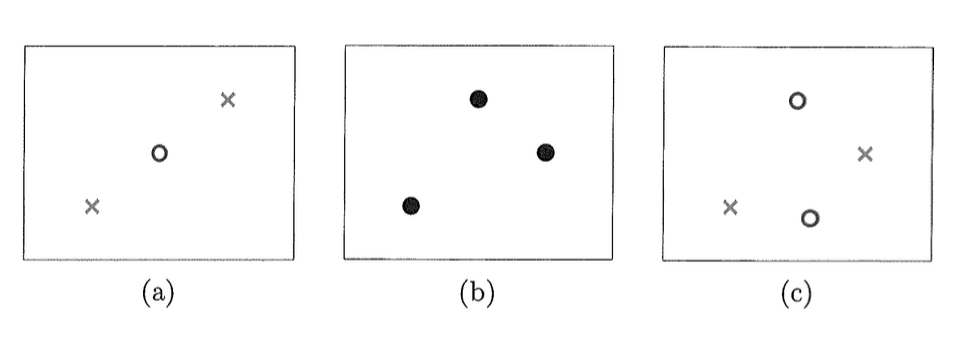
\includegraphics[width=0.8\textwidth]{Images/5.png}
    
    \caption{Fragmentación de muestras en $\mathbb{R}^2$ de tres y cuatro puntos.}
    \label{fragmentacion perceptron}
    \end{figure}

Es claro que no es posible separar de todas las maneras posibles a esta muestra en particular, por lo que su conjunto de fragmentación
tiene un cardinal menor a $2^3=8$. Pero sí es posible hacerlo con otras muestras de tres elementos, como por ejemplo cualquiera que tenga 
tres puntos no colineales, como en la figura \ref{fragmentacion perceptron} (b). De esto sigue
que los clasificadores lineales de este tipo tienen un coeficiente de fragmentación máximo de $2^3=4$ para muestras de tres puntos en $\mathbb{R}^2$.
Pero notemos que no es así cuando tomamos una muestra de cuatro puntos en $\mathbb{R}^2$. En este caso, es imposible separar de todas las maneras posibles
a una muestra de cuatro puntos, sean colineales o no, como se aprecia en la parte (c) de la figura. Demostraremos estos hechos más adelante.
\\

El coeficiente de fragmentación es una medida de la capacidad de una clase de funciones, es decir, mide 
el tamaño o la \textit{complejidad} de \(\mathcal{F}\) en un sentido particular. Si \(\mathcal{F}\) contiene muchas funciones, entonces 
$\mathcal{N}(\mathcal{F}, n)$ tiende a ser grande. Sin embargo, el coeficiente de fragmentación también tiene en cuenta 
la relación entre \(\mathcal{F}\) y el espacio de entrada de donde provienen los puntos de muestra. Más aún, nos permite asignar un número
finito a cada espacio de clasificadores para cada tamaño de muestras, aún cuando los espacios de funciones sean infinitos. Este número puede
ser en el peor de los casos exponencial en el tamaño de la muestra, pero nos ayudará a pasar del factor $m$, que depende de la cantidad
de funciones en el espacio (en la ecuación \ref{eq: chernoff acotada por m}), a un valor que es finito y, como veremos más adelante,
potencialmente polinómico.

\subsection{Cotas de convergencia uniforme}

Mantenemos la atención sobre la ecuación (\ref{eq:med_unif_riesgo_riesgo_emp}). Dado un espacio de funciones arbitrario, 
posiblemente infinito, ahora queremos analizar la probabilidad 
de que el riesgo empírico difiera significativamente del riesgo verdadero. Con las herramientas anteriores, 
podemos derivar una cota como sigue. Consideremos una muestra de \(2n\) puntos, es decir, un conjunto 
\(Z_{2n}\), donde interpretamos los primeros \(n\) puntos como la muestra original y los otros \(n\) 
puntos como la muestra fantasma.\\

La idea es reemplazar el supremo sobre \(\mathcal{F}\) en términos de \(R(f)\) y 
\(R_{\text{emp}}(f)\) por un supremo sobre los riesgos empíricos calculados en ambas muestras, es decir, por un expresión
que utilice el supremo sobre \(\mathcal{F}_{Z_{2n}}\). En este espacio, existen a lo sumo $\mathcal{N}(\mathcal{F}, n)<2^{2n}$
funciones distintas, lo que nos permite reemplazar, como indicabamos, el valor potencialmente infinito $m$ por el coeficiente de 
fragmentación. Escribimos:

\[
\begin{aligned}
P\left(\sup_{f \in \mathcal{F}} |R(f) - R_{\text{emp}}(f)| > \epsilon\right) &\leq 
2P\left(\sup_{f \in \mathcal{F}} |R_{\text{emp}}(f) - R'_{\text{emp}}(f)| > \frac{\epsilon}{2}\right).\\
& = 2P\left(\sup_{f \in \mathcal{F}_{Z_{2n}}} |R_{\text{emp}}(f) - R'_{\text{emp}}(f)| > \frac{\epsilon}{2}\right).\\
& \leq  \mathcal{N}(\mathcal{F}, n)\cdot \exp\left(\frac{-n\epsilon^2}{4}\right).
\end{aligned}
\]

Primero, utilizando el argumento de simetrización, como antes. Luego, el supremo puede restringirse a un conjunto finito de funciones
dado que estamos considerando solo los riesgos empíricos sobre dos muestras de tamaño $n$, que consideramos fijas, y de allí igualamos
en el segundo paso. Por último, aplicamos la cota de Chernoff (\ref{eq:Chernoff}), sabiendo que el numero de funciones
posibles $m$ es a lo sumo el coeficiente de fragmentación.\\

Para formalizar esto, usamos el coeficiente de fragmentación \(\mathcal{N}(\mathcal{F}, 2n)\), que proporciona el número máximo 
de particiones que \(\mathcal{F}\) puede realizar sobre una muestra de \(2n\) puntos. Aplicando el límite de la unión 
y la cota de Chernoff, obtenemos:

\begin{equation} 
    P\left(\sup_{f \in \mathcal{F}} |R(f) - R_{\text{emp}}(f)| > \epsilon \right) \leq 
    2\mathcal{N}(\mathcal{F}, 2n) \exp\left(-\frac{n\epsilon^2}{4}\right). \label{eq: cota convergencia coeficiente fragmentacion}
\end{equation}

Esta es una cota de convergencia uniforme que conecta el coeficiente de fragmentación con la probabilidad de 
que el riesgo empírico se desvíe significativamente del riesgo verdadero. Para que la minimización del riesgo 
empírico sea consistente, es suficiente que $\mathcal{N}(\mathcal{F}, n)$ crezca a un ritmo razonablemente lento, por ejemplo, 
polinomialmente en \(n\).\\

Tomemos $\mathcal{F}_{all}$, el espacio de todos los clasificadores posibles. Es claro que, en este caso, $\mathcal{N}(\mathcal{F}_{all}, n)=2^{2n}$,
pues cualquier muestra de $2n$ puntos puede ser separada de $2^{2n}$ formas posibles. Entonces, la cota de convergencia uniforme para este espacio
es:

\[
P\left(\sup_{f \in \mathcal{F}_{all}} |R(f) - R_{\text{emp}}(f)| > \epsilon \right) \leq
2\cdot 2^{2n} \exp\left(-\frac{n\epsilon^2}{4}\right) = 2\exp\left(n\left( 2\log(2) - \frac{n\epsilon^2}{4}\right)\right).
\]

Que es una expresión que no tiende a $0$ cuando $n$ tiende a infinito. Con lo que sabemos hasta ahora, esto no significa que podamos 
concluir que la minimización del riesgo empírico
usando el espacio de todas las funciones clasificadoras posibles sea inconsistente, dado que la cota de convergencia uniforme anterior
es solo una condicion suficiente. Pero si podemos dar el siguiente resultado para definir una condición necesaria y suficiente para
la consistencia de la minimización del riesgo empírico.
\begin{thm}
    La minimización del riesgo empírico es consistente con respecto a un espacio de funciones $\mathcal{F}$ si y solo si
    \[
    \frac{\log\left(\mathcal{N}(\mathcal{F}, n)\right)}{n} \rightarrow 0 \qquad \text{cuando } n \to \infty.
    \]
    
\end{thm}
\begin{proof}
    cf Mendelson 2003. Para teoremas relacionados, ver Vapnik y Chernovenkis 1971,1981, section 12.4, Devroye et al 1996.\\
\end{proof}

\begin{cor}
    Si $\mathcal{N}(\mathcal{F}, n)$ es polinómica, entonces la minimización del riesgo empírico es consistente con respecto a $\mathcal{F}$.\\
\end{cor}
\begin{cor}
    Si $\mathcal{N}(\mathcal{F}, n)=2^n$, entonces la minimización del riesgo empírico no es consistente con respecto a $\mathcal{F}$. En 
    particular, no es consistente con respecto al espacio de todas los clasificadores posibles $\mathcal{F}_{all}$.
\end{cor}

\subsection{Cotas de generalización}

Es a veces útil reescribir la ecuación (\ref{eq: cota convergencia coeficiente fragmentacion}) de forma inversa. Es decir, en lugar de 
fijar \(\epsilon\) y 
luego calcular la probabilidad de que el riesgo empírico se desvíe del riesgo verdadero en más de \(\epsilon\), 
podemos especificar la probabilidad con la que queremos que la cota se cumpla, y luego obtener una afirmación 
que nos indique qué tan cerca podemos esperar que esté el riesgo del riesgo empírico. Es decir, fijamos \(\delta > 0\) 
y resolviendo para \(\epsilon\). Como resultado, obtenemos que, con una probabilidad al menos \(1 - \delta\), cualquier 
función \(f \in \mathcal{F}\) satisface:

\begin{equation}
    R(f) \leq R_{\text{emp}}(f) + \sqrt{\frac{4}{n} \log(2\mathcal{N}(\mathcal{F}, n)) - \log(\delta)}. \label{eq: cota generalizacion}
\end{equation}


De la misma manera que antes, podemos usar esta cota para derivar afirmaciones de consistencia. Por ejemplo, 
ahora es evidente que la minimización del riesgo empírico es consistente para la clase de funciones \(\mathcal{F}\) 
si el término \(\log(2\mathcal{N}(\mathcal{F}, 2n))/n\) converge a \(0\) cuando \(n \to \infty\). Una vez más, 
este es el caso si \(\mathcal{N}(\mathcal{F}, 2n)\) crece de manera polinómica con \(n\).\\

Nótese que la cota (\ref{eq: cota generalizacion}) se cumple para todas las funciones \(f \in \mathcal{F}\). 
Por un lado, esto es una fortaleza 
de la cota, ya que se cumple en particular para la función \(f_n\) que minimiza el riesgo empírico, que es lo que 
buscamos. Además, muchos algoritmos de aprendizaje no minimizan exactamente el riesgo empírico, por lo que la cota 
también se cumple para ellos. Sin embargo, esto también puede interpretarse como una debilidad, ya que, al considerar 
un espacio más grande del necesario, obtenemos una cota menos ajustada de lo que podríamos si solo considerásemos
funciones en el espacio del algoritmo de aprendizaje..\\

Intentemos obtener una intuición sobre esta cota. Nos dice que si tanto \(R_{\text{emp}}(f)\) como el término 
de raíz cuadrada son pequeños simultáneamente, entonces podemos garantizar que, con alta probabilidad, el 
riesgo (es decir, el error en puntos futuros que aún no hemos visto) será pequeño. Esto puede parecer una 
afirmación sorprendente, sin embargo, no afirma nada imposible. Si usamos una clase de funciones con un 
\(\mathcal{N}(\mathcal{F}, n)\) relativamente pequeño, es decir, una clase de funciones que no puede explicar 
muchas funciones posibles, y luego notamos que usando una función de esta clase podemos explicar los datos muestreados 
del problema en cuestión, entonces es probable que esto no sea una coincidencia y hayamos capturado algunos aspectos 
esenciales del problema. \\

Por otro lado, si el problema es demasiado difícil de aprender a partir de la cantidad de datos dada, entonces 
descubriremos que, para explicar los datos (es decir, para lograr un \(R_{\text{emp}}(f)\) pequeño), necesitamos 
una clase de funciones que sea tan grande que pueda, en esencia, explicar cualquier cosa. En ese caso, el término 
de raíz cuadrada sería grande. Finalmente, nótese que la dificultad de aprender un problema está completamente 
determinada por si podemos encontrar una clase de funciones adecuada y, por lo tanto, por nuestro conocimiento 
previo sobre él. Incluso si la función óptima es subjetivamente muy compleja, si nuestra clase de funciones 
contiene esa función y pocas o ninguna otra, estamos en una excelente posición para aprender.\\

Existe una gran cantidad de cotas similares a (\ref{eq: cota convergencia coeficiente fragmentacion}) 
y su forma alternativa (\ref{eq: cota generalizacion}). Las diferencias ocurren en 
las constantes, tanto en el coeficiente frente a la exponencial como en su exponente. Las cotas también 
difieren en el exponente de \(\epsilon\) y en la forma en que miden la capacidad. \\

\subsection{La dimensión VC}

Hasta ahora hemos definido cotas de generalización en términos del coeficiente de framentación.
Aunque este es útil, a menudo es difícil calcularlo para clases de funciones arbitrarias. Existen otras medidas de capacidad
que son más fáciles de calcular y que proporcionan cotas más ajustadas, con ventajas y desventajas.
Introducimos la más conocida de todas, la llamada \textbf{dimensión VC} (dimensión de Vapnik-Chervonenkis). En pocas palabras,
esta medida intenta caratecterizar el crecimiento del coeficiente de fragmentación a medida que $n$ crece, destilado en un 
solo valor.\\

Decimos que una muestra \(Z_n\) de tamaño \(n\) es fragmentada por la clase de funciones 
\(\mathcal{F}\) si \(\mathcal{N}(\mathcal{F}, n) = 2^n\). Es decir, \(\mathcal{F}\) puede realizar cualquier separación posible de etiquetas sobre 
los puntos de la muestra. La dimensión VC de \(\mathcal{F}\), denotada como \(\text{VC}(\mathcal{F})\), se define como el tamaño 
máximo de una muestra que puede ser fragmentada por \(\mathcal{F}\). Formalmente:\\

\begin{dfn}
La dimensión VC de una clase de funciones \(\mathcal{F}\) es el tamaño máximo de una muestra que puede ser fragmentada por \(\mathcal{F}\), es decir:
\[
\text{VC}(\mathcal{F}) = \max \{n \in \mathbb{N} \mid \mathcal{N}(\mathcal{F}, n) = 2^n\}.
\]
Si no existe tal máximo, definimos \(\text{VC}(\mathcal{F}) = \infty\). \\
\end{dfn}

La dimensión VC tiene una interpretación combinatoria 
elegante y proporciona una forma práctica de analizar la capacidad de \(\mathcal{F}\). Por ejemplo, si \(\text{VC}(\mathcal{F})\) 
es finita, podemos garantizar la consistencia de la minimización del riesgo empírico. Además, una clase de funciones 
con dimensión VC más baja tiende a tener una mejor capacidad de generalización.\\

\begin{lem}
    Sea $\mathcal{F}$ una clase de funciones con dimensión VC finita. Entonces
    \[
    \mathcal{N}(\mathcal{F}, n) \leq \sum_{i=0}^{\text{VC}(\mathcal{F})} \binom{n}{i} , \qquad \forall n \in \mathbb{N}.
    \]
    En particular, para $n\geq \text{VC}(\mathcal{F})$ se tiene que 
    \[
    \mathcal{N}(\mathcal{F}, n) \leq \left(\frac{e\cdot n}{\text{VC}(\mathcal{F})}\right)^{\text{VC}(\mathcal{F})}.
    \]
\end{lem}

La importancia de esta afirmación radica en el último hecho. Si \( n \geq \text{VC}(\mathcal{F}) \), 
el coeficiente de fragmentación se comporta como una función polinómica del tamaño de la muestra \( n \). 
Este es un resultado muy notable: una vez que sabemos que la dimensión VC de una clase de funciones 
\(\mathcal{F}\) es finita, ya sabemos que los coeficientes de fragmentación crecen polinómicamente con \( n \). 
Por los resultados de la sección anterior, esto implica la consistencia de la minimización del riesgo empírico.\\
Nótese que también tenemos una afirmación en la otra dirección. Si la dimensión VC es infinita, esto significa 
que para cada \( n \) existe alguna muestra que puede ser fragmentada por \(\mathcal{F}\), es decir, tal que
\(\mathcal{N}(\mathcal{F}, n) = 2^n. \) Para este caso, ya vimos anteriormente que ERM no es consistente.\\
Enunciamos todo esto en el siguiente Teorema.\\

\begin{thm}
    La minimización del riesgo empírico es consistente con respecto a una clase de funciones \(\mathcal{F}\) si y solo si
    \(\text{VC}(\mathcal{F}) < \infty\).\\ 
\end{thm}

Una propiedad importante a notar tanto sobre el coeficiente de fragmentación como sobre la 
dimensión VC es que no dependen de la distribución subyacente \( P \), sino únicamente de la 
clase de funciones \(\mathcal{F}\). Por un lado, esto es una ventaja, ya que todas las cotas de 
generalización derivadas de estos conceptos se aplican a todas las distribuciones de probabilidad 
posibles. Por otro lado, esto también puede considerarse una desventaja, ya que los conceptos de 
capacidad no tienen en cuenta propiedades particulares de la distribución en cuestión. En este 
sentido, estos conceptos de capacidad a menudo conducen a cotas bastante amplias, pero es lo que desde
un comienzo nos interesaba.\\

\subsection{Complejidad de Rademacher}
Un concepto diferente para medir la capacidad de un espacio funcional es la \textbf{complejidad de Rademacher}. 
En comparación con el coeficiente de fragmentación y la dimensión VC, esta sí depende de la distribución de 
probabilidad subyacente y, por lo general, conduce a cotas mucho más ajustadas que ambas. \\

La complejidad de Rademacher se define de la siguiente manera.

\begin{dfn}
Sean \(\sigma_1, \sigma_2, \dots\) variables aleatorias independientes que toman los valores \(+1\) y \(-1\) 
con probabilidad \(0.5\). Definimos la complejidad de Rademacher \(\mathscr{R}(\mathcal{F})\) de un espacio funcional 
\(\mathcal{F}\) como:

\[
    \mathscr{R}(\mathcal{F}) := \mathbb{E} \sup_{f \in \mathcal{F}} \frac{1}{n} \sum_{i=1}^{n} \sigma_i f(X_i).
\]
\end{dfn}

Cada una de estas variables aleatorias se denominan \textit{variables de Rademacher}. 
Por ejemplo, pueden interpretarse como los resultados de lanzar repetidamente una moneda no cargada. 

Consideremos primero los valores \(\sigma_i\) como fijos e interpretémoslos como etiquetas asignadas a los puntos \(X_i\). Como tanto 
\(\sigma_i\) como \(f(X_i)\) solo toman los valores \(+1\) o \(-1\), el producto \(\sigma_i f(X_i)\) toma el 
valor \(+1\) si \(\sigma_i = f(X_i)\), y \(-1\) si \(\sigma_i \neq f(X_i)\). \\

Como consecuencia, la suma en el lado derecho de la ecuación será grande si las etiquetas \(f(X_i)\) 
coinciden con las etiquetas \(\sigma_i\) en muchos puntos de datos. Esto significa que la función \(f\) 
se ajusta bien a las etiquetas \(\sigma_i\): si las etiquetas \(\sigma_i\) fueran en general correctas, 
\(f\) tendría un error de entrenamiento (o riesgo empírico) pequeño. Luego

\[
\sup_{f \in \mathcal{F}} \sum_{i=1}^{n} \sigma_i f(X_i)
\]

es grande si existe una función en \(\mathcal{F}\) que se ajusta bien a la secuencia dada de etiquetas \(\sigma_i\). \\

Ahora recordemos que las etiquetas \(\sigma_i\) son variables aleatorias. Podemos considerarlas 
como etiquetas aleatorias asignadas a los puntos de datos \(X_i\). Como tomamos la esperanza sobre ambos, los 
puntos de datos y las etiquetas aleatorias, la complejidad de Rademacher será alta si el espacio funcional 
\(\mathcal{F}\) es capaz de ajustarse bien a etiquetas aleatorias. Esta intuición tiene sentido: un espacio 
funcional debe ser bastante grande para poder ajustarse a todo tipo de etiquetas aleatorias en todo tipo de 
conjuntos de datos. En este sentido, la complejidad de Rademacher mide qué tan complejo es el espacio 
funcional: cuanto mayor sea \(\mathscr{R}(\mathcal{F})\), mayor será la complejidad de \(\mathcal{F}\).\\

Desde un punto de vista matemático, la complejidad de Rademacher es conveniente para trabajar. Se pueden 
demostrar cotas de generalización de la siguiente forma:
\begin{thm}
    Sea $\mathcal{F}$ un espacio funcional y $Z_n$ una muestra de tamaño $n$. Entonces, para cualquier $\delta > 0$,
\[
\mathcal{R}(f) \leq \mathcal{R}_{\text{emp}}(f) + 2\mathscr{R}(\mathcal{F}) + \sqrt{\frac{\log(1/\delta)}{2n}}.
\]
con probabilidad al menos \(1 - \delta\).\\
\end{thm}


La complejidad de Rademacher tienen algunas ventajas sobre los conceptos clásicos de capacidad, como la 
dimensión VC. En particular, las cotas obtenidas mediante complejidades de Rademacher tienden a ser mucho más 
precisas que las obtenidas mediante herramientas clásicas. Las técnicas de demostración son diferentes de las 
explicadas anteriormente, pero no entraremos en detalles aquí. Para literatura sobre cotas basadas en la 
complejidad de Rademacher, véase, por ejemplo, Mendelson (2003), Bousquet et al. (2003) o Boucheron et al. 
(2005) y las referencias allí citadas.\\

\subsection{Cotas con grandes márgenes de separación}

Finalmente, queremos introducir otro tipo de medida de capacidad de clases de funciones que es 
más especializada que las cantidades combinatorias generales presentadas anteriormente. Consideremos 
el caso particular en el que el espacio de datos consiste en puntos en el espacio bidimensional 
\(\mathbb{R}^2\) y donde queremos separar las clases mediante una línea recta. Dado un conjunto 
de puntos de entrenamiento y un clasificador \(f_n\) que puede separarlos perfectamente, definimos 
el \textbf{margen} del clasificador \(f_n\) como la menor distancia de cualquier punto de entrenamiento 
a la línea separadora definida por \(f_n\) (véase la Figura 5). De manera análoga, se puede definir 
un margen para clasificadores lineales en un espacio de dimensión arbitraria \(d\).

\begin{figure}[h!]
    \centering
    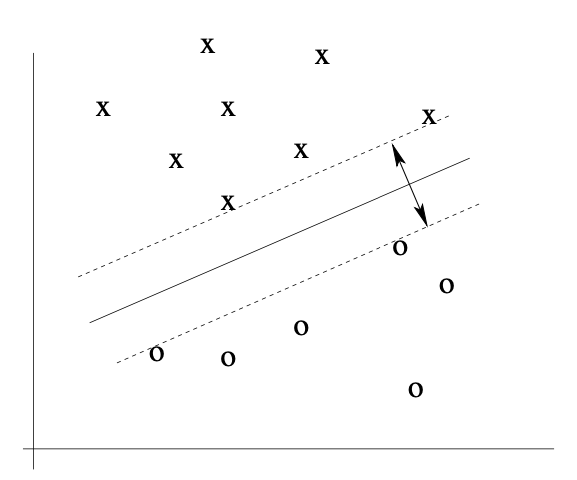
\includegraphics[width=0.5\textwidth]{Images/6.png}
    \caption{Margen de un clasificador lineal: las cruces representan puntos de entrenamiento con 
    etiqueta \(+1\), mientras que los círculos representan puntos de entrenamiento con etiqueta \(-1\). 
    La línea recta es el clasificador lineal \(f_n\), y la línea discontinua muestra el margen. La 
    anchura \(\rho\) del margen está representada por la flecha.}
    \label{fig:Clasificación con margen}
\end{figure}

Se puede demostrar que la dimensión VC de la clase \(\mathcal{F}_\rho\) de funciones lineales con 
margen al menos \(\rho\) puede ser acotada esencialmente por la razón entre el radio \(R\) de la 
esfera más pequeña que encierra los puntos de datos y el margen \(\rho\), es decir,

\[
\text{VC}(\mathcal{F}_\rho) \leq \min \left(d, \frac{4R^2}{\rho^2} + 1 \right).
\]

(cf. Teorema 5.1 en Vapnik, 1995). Es decir, cuanto mayor sea el margen \(\rho\) de las funciones 
en la clase \(\mathcal{F}_\rho\), menor será su dimensión VC. De esta manera, se puede usar el 
margen de los clasificadores como un concepto de capacidad. Uno de los clasificadores más conocidos, 
la \textbf{máquina de soporte vectorial} (SVM, \textit{Support Vector Machine}), se basa en este 
resultado. Para un tratamiento más completo, véase Schölkopf y Smola (2002).

Un ejemplo de cota de generalización que involucra el gran margen es el siguiente (para una 
declaración más precisa, véase el Teorema 7.3 en Schölkopf y Smola, 2002):

\begin{thm}[Cotas de grandes márgenes]

Supongamos que el espacio de datos está contenido dentro de una esfera de radio \(R\) en 
\(\mathbb{R}^d\). Consideremos el conjunto \(\mathcal{F}_\rho\) de clasificadores lineales con 
margen al menos \(\rho\). Supongamos que se nos dan \(n\) ejemplos de entrenamiento. Denotemos 
por \(\nu(f)\) la fracción de ejemplos de entrenamiento con margen menor que \(\rho\) o que han 
sido clasificados erróneamente por algún clasificador \(f \in \mathcal{F}_\rho\). Entonces, con 
probabilidad al menos \(1 - \delta\), el error verdadero de cualquier \(f \in \mathcal{F}_\rho\) 
puede ser acotado por:

\[
\mathcal{R}(f) \leq \nu(f) + \sqrt{\frac{c}{n} \left( \frac{R^2}{\rho^2} \log(n)^2 + \log(1/\delta) \right)} .
\]
\end{thm}


\bigbreak
\pagebreak
\section{Bibliografía}

[1] \textit{Statistical Learning Theory: Models, Concepts and Results} - von Luxburg, Schölkopf (2008). \\

[2] \textit{The Nature of Statistical Learning Theory} - Vladimir Vapnik (1995). \\

[3] \textit{Statistical Learning Theory} - Vladimir Vapnik (1998). \\

[4] \textit{A Probabilistic Theory of Pattern Recognition} - Luc Devroye, László Györfi, Gábor Lugosi (1996). \\

[5] \textit{Learning with Kernels} - B. Schölkopf, A. Smola (1996). \\

[6] \textit{Statistical Inference} - Casella, Berger . \\

[7] \textit{Pattern Recognition and Machine Learning} - C. Bishop (2006). \\





\end{document}